  
\chapter{基于AI基础模型微调的变化检测模型研究}

在计算机视觉领域,许多深度学习模型依赖于在 ImageNet 等自然场景数据集上的大规模预训练。然而,自然场景图像与遥感影像之间存在显著差异。如图~\ref{fig:changeclip2}所示,前者通常来自水平或倾斜视角拍摄,呈现明显的透视效应和单一目标结构。而后者多为垂直俯视获取,涵盖范围广泛、尺度跨度大,且地物之间紧密排列。此外,遥感影像还具有多源、多分辨率、多时相等特性,这些因素使得直接将基于 ImageNet 预训练的模型迁移到遥感任务中往往存在域偏移现象。随着现如今 AI 基础模型的发展,一些基础模型通常会基于海量样本进行训练。比如,CLIP模型~\cite{Radford2021LearningTV}包含 4 亿(400 million)图像‑文本对用于自监督训练。SAM 模型~\cite{Kirillov2023SegmentA}包含1100 万分割图像数据,涉及到11 亿个分割掩码,用于创建大型的图像分割模型。DINOv2~\cite{Oquab2023DINOv2LR} 于 2023 年训练时使用了 1 亿 4 千万张无标签图像进行自监督训练,最新的 DINOv3~\cite{simeoni2025dinov3} 训练规模进一步扩大,训练数据集达到 170 亿 图像规模。因此,此类的 AI 基础模型通常具有非常强大的数据泛化能力,同时针对遥感影像也具有极强的无监督泛化能力。为此,在本章中,本章针对遥感场景特点开展基于 AI 基础模型的变化检测研究。具体而言,本章一方面探索了结合 CLIP 架构的多模态变化检测模型,另一方面探索了如何通过参数高效微调与领域自适应策略,使视觉基础预训练模型能够更好地适配遥感数据特性,从而提升在多源、多尺度和多时相条件下的遥感影像变化检测性能。

\section{基于多模态架构的变化检测方法}
\subsection{结合多模态的变化检测方法概述}

在遥感影像变化检测(Remote Sensing Change Detection,RSCD)领域,Siamese神经网络是最流行的基线方法~\cite{Koch2015SiameseNN, Wang2022AnES}。Siamese神经网络采用并行结构,具有两个相同的子网络,可以提取稳健且具辨识性的特征,并直接输出变化结果。基于这一结构,许多变化检测方法应运而生,有的应用卷积神经网络(CNN)~\cite{chen2023continuous, Tian2022LargescaleDL, zhu_land-useland-cover_2022-1},有的采用Transformer架构~\cite{chen_remote_2022, Li2022TransUNetCDAH, Liu2022RemoteSI}。然而,这些方法仅考虑了单一模态的数据,即图像,而忽视了多模态数据中的丰富语义信息,因此面临瓶颈。为了解决这些限制,探索一个基于基础模型的多模态RSCD框架是十分必要的。

近年来,视觉-语言表征学习成为计算机视觉中的一个热门研究课题,该方法通过深度学习模型从图像-文本对中学习表征。得益于这种模式,这种方法已在许多多模态任务中取得了进展,如图像描述~\cite{Chen2021VisualGPTDA}、视觉问答~\cite{Song2022CLIPMA}和跨模态检索~\cite{Tang2023InteractingEnhancingFT}。例如,Visual-BERT模型扩展了BERT~\cite{Devlin2019BERTPO},通过双流结构对图像和文本进行编码,并从多模态层捕获丰富的语义信息。在遥感领域,Rahhal等人~\cite{AlRahhal2022MultilanguageTF}采用Transformer网络作为编码器,处理图像和文本描述,用于精确的遥感图像检索。Liu等人~\cite{Liu2022RemoteSI}提出了LEVIR变化描述数据集,并引入文本描述表示遥感图像中的变化区域。特别地,CLIP~\cite{Radford2021LearningTV}通过图像-文本对的对比学习,展示了强大的图像识别能力和显著的零-shot适应性。

\begin{figure}[!htbp]
  \centering
  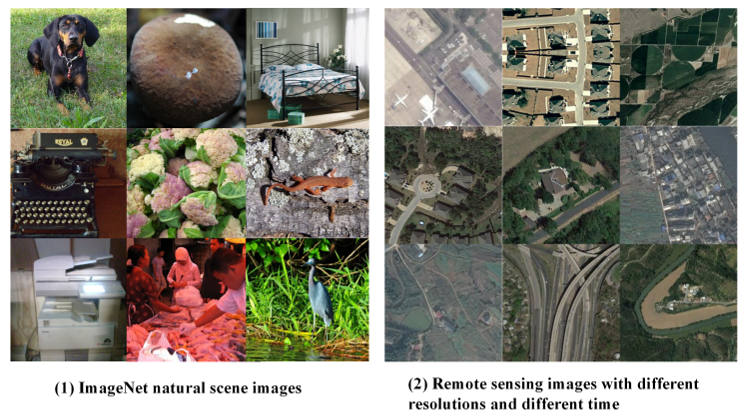
\includegraphics[width=\textwidth]{paper_figures/基于AI基础模型微调的变化检测模型研究/ChangeCLIP/changeclip2.png}
  \caption{ImageNet自然场景图像与遥感图像的比较.}
  \label{fig:changeclip2}
\end{figure}

\begin{figure}[!htbp]
  \centering
  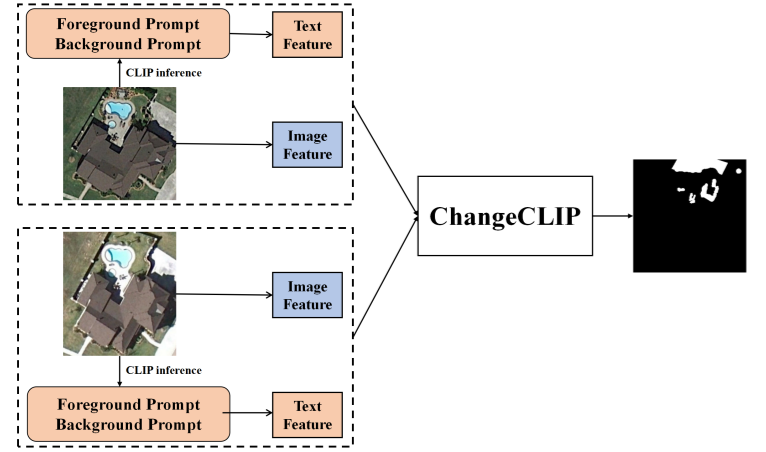
\includegraphics[width=\textwidth]{paper_figures/基于AI基础模型微调的变化检测模型研究/ChangeCLIP/changeclip1.png}
  \caption{多模态遥感变化检测架构.}
  \label{fig:changeclip1}
\end{figure}




本节将CLIP引入RSCD任务,并提出了一个多模态变化检测框架,命名为ChangeCLIP,如图~\ref{fig:changeclip1}所示。在多模态变化检测任务中,通常使用单一模态,主要是遥感影像,来识别变化。为了结合基于文本的提示信息,利用CLIP模型基于56个常见的地表覆盖分类生成描述性提示,如表I所示。这些分类涵盖了遥感数据集中常见的目标元素。本节进一步将这56种类型归类为更广泛的分类,以便参考,如表~\ref{tab:remote_sensing_categories}所示。如图~\ref{fig:changeclip2}的文本框所示,为遥感图像的前景和背景特征设计了特定的提示,利用CLIP模型作为基础。通过这种方式,构建了一个基本数据集,丰富了用于变化检测任务的多模态先验信息。在图像编码阶段,本节构建了一个Siamese神经网络,从双时相遥感影像中提取图像特征。在文本编码阶段,本节应用Transformer网络从文本提示中提取文本特征。为了充分利用多模态特征学习的优势,本节在ChangeCLIP中有效地结合了视觉和文本特征。此外,本节提出了一种新颖的差异特征补偿(Differential Feature Compensation,DFC)模块,用于输出语义变化。


\begin{table}[!htbp]
  \centering
  \caption{遥感影像中的常见地物类别}
  \label{tab:remote_sensing_categories}
  \begin{tabularx}{\linewidth}{@{}l X@{}}
    \toprule
    Category                      & Items \\
    \midrule
    Natural Environment           & Beach, Forest, Lake, Meadow, Mountain, Sea, Wetland, Cotton Field, Farmland, Prairie, Desert, River, Tree, Shrubbery, Chaparral, Fertile Land, Snow Land, Pond, Island \\
    \midrule
    Transportation                & Airport, Bridge, Freeway, Harbor, Railway, Interchange, Intersection, Road, Highway \\
    \midrule
    Recreation \& Sports          & Basketball Court, Ground Track Field, Stadium, Tennis Court, Golf Course \\
    \midrule
    Residential \& Buildings      & Dense Residential, Single-Family Residential, Building, Church, Cabin \\
    \midrule
    Commercial \& Industrial      & Commercial Area, Industrial Area, Oil Tank, Storage Tanks, Container, Mine \\
    \midrule
    Other Man-made Structures     & Terrace, Campus, Park, Parking Lot, Square, Solar Panel, Cars, Ship, Airplane, Runway, Impermeable Surface \\
    \bottomrule
  \end{tabularx}
\end{table}

\subsection{ChangeCLIP网络设计}
\subsubsection{ChangeCLIP总体结构设计}
本节提出了一种创新的方法ChangeCLIP,利用大规模视觉-语言模型来处理遥感变化检测(RSCD)任务。如图~\ref{fig:changeclip3}所示,ChangeCLIP的综合框架分为四个主要部分:多模态数据、多模态编码器、差异特征补偿和视觉-语言驱动解码器。在第一个部分,利用CLIP模型的无监督分类能力为遥感影像生成文本提示,从而构建多模态输入数据,用于变化检测任务。第二部分,采用CLIP模型构建图像和文本编码器,作为多模态RSCD任务的基础双时相特征提取器。此外,将图像特征与文本特征相结合,有效补偿了传统单模态变化检测方法中的局限性。第三部分,为了增强模型捕捉双时相变化的能力,引入了差异特征补偿(DFC)模块。该模块利用多种计算方法表示差异特征,并通过特征图的加权融合,优化了对不同双时相影像差异的适应能力。在最后一个部分,充分利用从编码阶段获得的视觉-语言特征。通过将这些视觉-语言特征与解码阶段的特征相结合,设计了一个视觉-语言驱动的解码器。

\begin{figure}[!htbp]
  \centering
  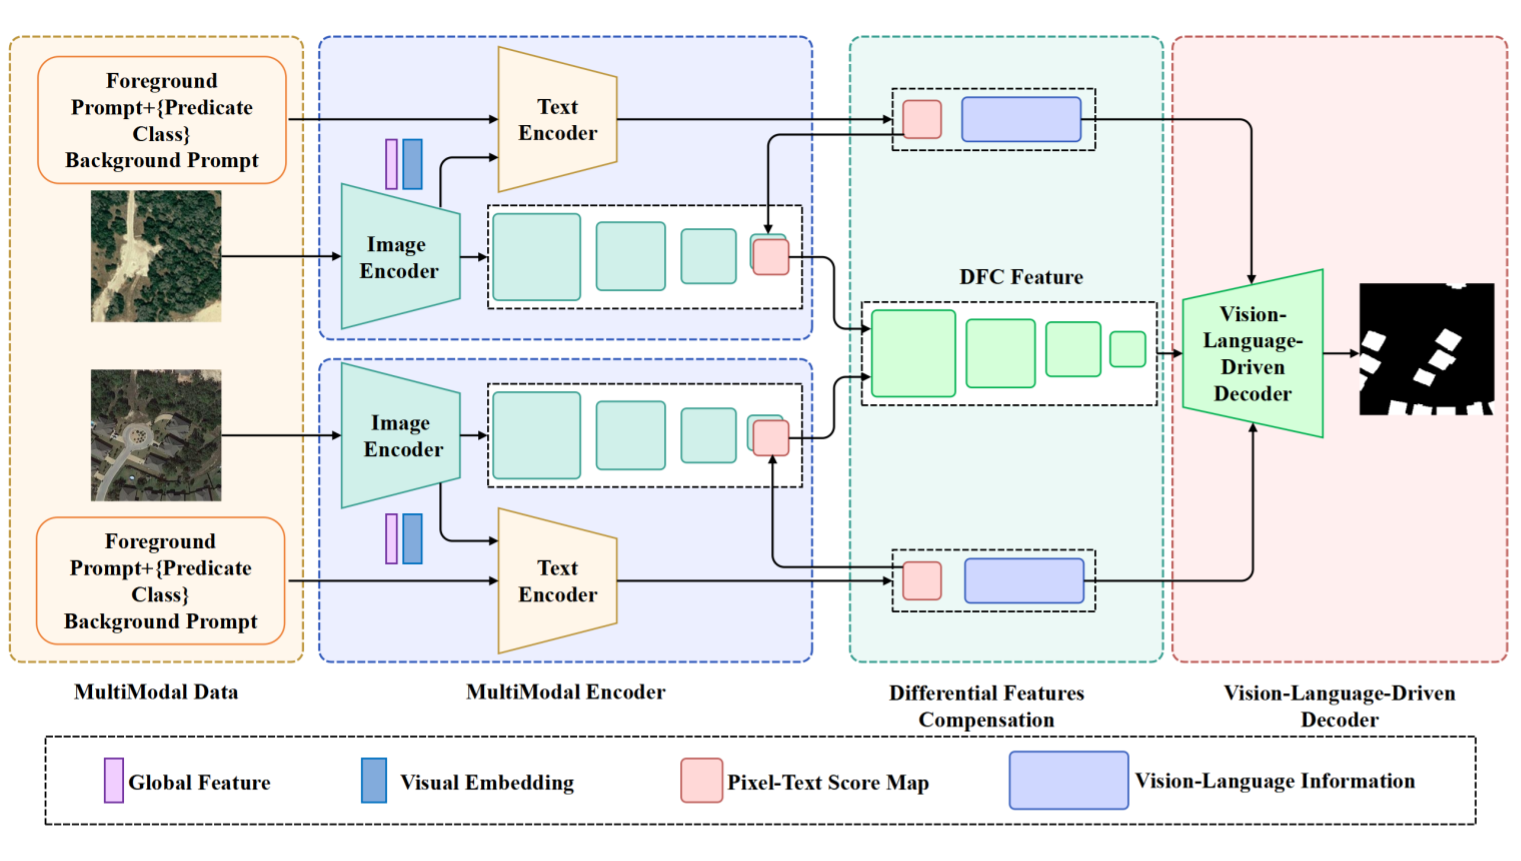
\includegraphics[width=\textwidth]{paper_figures/基于AI基础模型微调的变化检测模型研究/ChangeCLIP/changeclip3.png}
  \caption{ChangeCLIP 变化检测架构。Global Feature (全局特征) 是从图像中获取的、具有物体识别能力的特征信息。Visual Embedding (视觉嵌入) 是高层特征图,被视为图像的嵌入。Pixel-Text Score Map (像素-文本得分图) 是图像与文本提示之间的相关性图。Vision-Language Information (视觉-语言信息) 意味着结合了图像特征和文本特征。}\label{fig:changeclip3}
\end{figure}

\subsubsection{多模态编码器}
如今,计算机视觉和自然语言处理(NLP)越来越紧密地结合在一起,催生了许多将计算机视觉和NLP相结合的优秀项目~\cite{Chen2021VisualGPTDA, Lu2019ViLBERTPT}。在ChangeCLIP模型中,通过将CLIP的大规模图像-文本先验知识与变化检测相结合,提出了一种多模态遥感影像变化检测(RSCD)框架,如图\ref{fig:changeclip3}所示。由于当前没有像素级的变化检测数据集提供文本提示标签,本节利用CLIP的无监督预测能力来制定原始的遥感影像文本提示。具体而言,为了获得双时相影像的文本表示,本节使用CLIP模型对这56个类别进行预测,如表I所示。本节选择了具有最高置信度的9个类作为预测类别。因此,前景的文本描述设置为``遥感影像前景物体,\{预测类别\}'', 而``遥感影像背景物体''作为背景的文本描述。本节的目标是变化区域,因此使用预测类别组成前景的文本提示,正如上述所提到的那样。通过这种方式,变化物体可以通过双时相文本提示直接展示,而双时相文本提示提供了遥感先验知识。最终,ChangeCLIP的输入由两对并行的图像编码器和文本编码器组成。

图像编码器和文本编码器从 CLIP 模型的图像编码器和文本编码器中选取,以有效利用 CLIP 模型强大的图像–文本建模能力。在特征提取阶段,双流图像编码器获得两组特征金字塔$\{F_{a1},F_{a2},F_{a3},F_{a4}\}$ 和 $\{F_{b1},F_{b2},F_{b3},F_{b4}\}$,分别表示双时相的多级特征。在计算机视觉中,深度网络的特征维度较高且具有更强的判别能力,因此通常认为高层次图像特征能够表征图像的语义信息。因此,将高层次语义特征图与文本序列特征相结合。为了结合高层次语义特征图与文本序列特征,ResNet~\cite{He2015DeepRL}主干和 ViT~\cite{Dosovitskiy2020AnII}主干有所区别:在 ResNet 的情况下,使用注意力池化模块生成高层次语义特征,将其视为图像序列特征;而在 ViT 中,则直接将高层次特征作为图像序列特征。这种在 ViT 中的图像序列特征与文本序列特征的对齐有助于促进两种模态之间更紧密的表示。来自 ViT 主干的图像序列特征天然地与文本序列特征对齐,增强了模型捕捉两种模态内在关系和语义一致性的能力。相比 ResNet 主干,ViT 在多模态任务上通常具有更好的表征能力。以 ResNet 为例来描述该部分的计算步骤,因为 ResNet 的序列特征提取算法相较 ViT 更为复杂。视觉编码过程结束时,使用注意力池化模块对高层次特征图进行视觉嵌入,以构建图像序列特征。进一步地,在多模态特征提取阶段有效地结合图像信息和文本信息,共同更新多模态特征提取的权重。计算步骤如下:
\begin{align}
x_1 &= \mathrm{Reshape}(x) \label{eq:changeclip-1}\\
x_{\mathrm{avg}}(i,j) &= \frac{1}{HW}\sum_{h_w=1}^{HW} x(h_w, i, j) \label{eq:changeclip-2}\\
x_2 &= \mathrm{Concat}\bigl(x_{\mathrm{avg}}, x_1\bigr) \label{eq:changeclip-3}\\
x_3 &= x_2 + \mathrm{pos\_embedding} \label{eq:changeclip-4}\\
x_4 &= \mathrm{softmax}\!\Bigl(\frac{x_3 x_3^{\mathrm{T}}}{\sqrt{d_k}}\Bigr)\,x_3 \label{eq:changeclip-5}\\
x_5 &= \mathrm{Reshape}(x_4) \label{eq:changeclip-6}\\
\mathrm{global\_feature} &= x_5[:,:,0] \label{eq:changeclip-7}\\
\mathrm{visual\_embedding} &= \mathrm{Reshape}\bigl(x_5[:,:,1]\bigr) \label{eq:changeclip-8}
\end{align}

其中,$x\in\mathbb{R}^{n\times c\times h\times w}$ 表示 ResNet 在编码阶段提取的高层次特征图,包含了整个图像的高维语义信息;$n,c,h,w$ 分别表示批大小(batch size)、通道数、特征图的高度和宽度。$x_1\in\mathbb{R}^{hw\times nc}$ 将输入特征图从二维重塑为一维序列。$x_{\mathrm{avg}}$ 表示平均池化的结果,代表输入特征图的全局信息。将二维特征图重塑为一维序列会破坏像素间的空间关系,因此使用位置嵌入(pos\_embedding)来补充特征图的位置信息。如公式 \eqref{eq:changeclip-5} 所示,多头注意力模块用于处理带有全局信息的视觉序列特征图,产生 $\mathrm{global\_feature}\in\mathbb{R}^{n\times (c/2)}$ 和 $\mathrm{visual\_embedding}\in\mathbb{R}^{n\times (c/2)\times h\times w}$。$d_k$ 是用于调整注意力模块敏感度的缩放因子。$\mathrm{global\_feature}$ 表示原始输入图像的全局语义类别信息;$\mathrm{visual\_embedding}$ 是经过嵌入编码后的视觉特征图,可与后续的文本序列特征结合。为了适应变化检测双流网络的特性,分别提取双时相图像的特征,然后计算双时相图像的 $\mathrm{global\_feature}$ 和 $\mathrm{visual\_embedding}$。

为了更好地利用文本提示提供的语义信息与图像信息之间的关联,需要将文本编码特征与图像特征结合,以计算文本与图像结合后的特征序列。在 ChangeCLIP 中,图像序列特征由上述提到的 \(\mathrm{global\_feature}\) 和 \(\mathrm{visual\_embedding}\) 组成。从文本编码器获得的文本语义特征通过 Transformer 模块与图像的特征序列相结合。其计算步骤如下:
\begin{align}
t_2 &= F_{\mathrm{te}}(t_1) \label{eq:changeclip-9}\\
\hat t_2 &= F_{\mathrm{cd}}(t_2, V) \label{eq:changeclip-10}\\
t_3 &= t_2 + \gamma \times \hat t_2 \label{eq:changeclip-11}\\
\mathrm{score\_map} &= \eta(t_3)\times \eta(V') \label{eq:changeclip-12}
\end{align}

其中,\(t_1\) 是文本 token;\(F_{\mathrm{te}}\) 是基于 Transformer 的文本编码器;\(t_2\) 是 Transformer 生成的文本嵌入;\(V\) 表示将 \(\mathrm{global\_feature}\) 和 \(\mathrm{visual\_embedding}\) 结合后的特征表示;\(F_{\mathrm{cd}}\) 是图像特征序列与文本嵌入之间进行上下文解码的解码器;通过 \(F_{\mathrm{cd}}\) 的计算,图像特征序列和文本嵌入得以通过上下文解码器中的 Transformer 块有效结合,而 \(\hat t_2\) 是 \(F_{\mathrm{cd}}\) 的输出。在公式 \eqref{eq:changeclip-11} 中,通过可学习系数 \(\gamma\) 将 \(\hat t_2\) 与 \(t_2\) 相结合,以有效关联图像特征与文本特征。于是,包含文本与图像信息的 \(t_3\) 可以表征图像视觉特征与文本语义特征结合后的信息。因此,在解码阶段将 \(t_3\) 作为视觉–语言特征的补充,与解码中的视觉特征 \(V'\) 结合。\(V'\) 是在图像编码阶段从高层次语义特征计算得到的 \(\mathrm{visual\_embedding}\),\(\eta\) 是归一化函数。通过上述计算方法得到逐像素—文本的 \(\mathrm{score\_map}\)。\(\mathrm{score\_map}\) 表示图像视觉嵌入与文本特征序列之间的关系。在本节中,\(\mathrm{score\_map}\) 与图像特征提取中的高层次语义特征结合,以补充高层次语义特征中的文本相关语义信息,使高层次语义特征图更加具有判别力。

\subsubsection{结合余弦相似度计算的混合差异特征计算方法}

传统的变化检测方法通常基于语义分割来进行任务处理。然而,这种方法存在一个缺点,即忽略了任务中最重要的变化特征。变化检测的主要关注点是遥感影像在不同时间段的变化区域,而不是特定的语义类别。通过使用语义分割,重点在于将像素分类为不同的语义类别,这对于遥感影像中的变化检测并不适用。因此,遥感影像变化检测(RSCD)的核心在于模型对变化特征的表示能力。为了解决这个问题,提出了一种新型的差异特征补偿(DFC)模块,该模块基于不同时间段遥感影像的差异特征计算,如图4所示。通过DFC模块,网络可以专注于通过不同的特征计算模块学习双时相遥感影像的变化特征,而不是语义类别。因此,本节提出的方法比依赖语义分割的传统方法更能针对遥感影像的变化检测。

具体来说,双时相遥感影像在空间上表现出一致性,但在地理上存在时间差异。在这一阶段,常见的双时相特征融合策略是使用Concat计算方法。从深度学习的理论基础出发,Concat的计算方法只是将双时相特征图合并,差异特征的体现通过反向传播算法学习。在双时相特征融合中,Concat并没有突出差异特征在RSCD任务中的重要性。因此,我们考虑使用另外两种更直接的差异特征计算方法。对于双时相特征,特征的差异主要体现在两个方面,一方面是像素特征序列的数值差异,如减法。另一方面是基于余弦相似度的像素特征序列在高维空间中的语义差异。对于前者,简单的减法计算方法可以更好地表达高层特征图中的差异。但在低层特征图中,由于不同时间阶段的相同类型地物可能具有较大的颜色差异,减法计算方法很难准确表达变化特征。对于后者,余弦相似度可以有效捕捉高维向量的相似性。在双时相特征分析的背景下,余弦相似度弥补了减法在表示向量方向差异方面的不足。因此,从差异表示的角度来看,减法和余弦相似度是互补的。

基于上述分析,本节设计了用于差异学习的 DFC 模块。首先,通过特征图相减计算差异。由于算法的识别目标是变化区域,单纯的特征图相减结果无法充分表达该区域在语义上的特征。因此,为更好地适配双时相图像变化的特点,对相减结果取绝对值,以更好地表达通过相减获得的兴趣区域显著图,并引入卷积模块,使网络能够自适应地优化相减后的特征图。由此生成的特征图能够突出显示变化区域的特征。与此同时,考虑到余弦距离能够在高维空间中表示不同特征向量的相似性,设计了另一种基于余弦距离的特征差异计算模块。综上,DFC 的计算步骤如下:
\begin{align}
F_{\mathrm{sub}} &= \sigma\bigl(\lvert F_a - F_b\rvert\bigr) \label{eq:changeclip-13}\\
\varphi &= \frac{x_1 \cdot x_2}{\max\bigl(\lVert x_1\rVert_2 \cdot \lVert x_2\rVert_2,\ \varepsilon\bigr)},\quad x_1\in F_a,\ x_2\in F_b,\ \varepsilon=1\times10^{-8} \label{eq:changeclip-14}\\
m &= \varphi\bigl(1 - \varphi(F_a, F_b)\bigr) \label{eq:changeclip-15}\\
X &= \mathrm{FPN}\bigl(\mathrm{concat}(F_a, F_b)\bigr) \label{eq:changeclip-16}\\
\hat X &= \mathrm{CA}\bigl(\mathrm{concat}(X \times m,\ F_{\mathrm{sub}},\ X)\bigr) \label{eq:changeclip-17}
\end{align}

其中,$F_a$、$F_b$ 是融合了不同时相视觉–语言信息的特征图;$\sigma$ 表示卷积模块;$F_{\mathrm{sub}}$ 为特征图相减后取绝对值得到的差异图;$\varphi$ 表示余弦相似度计算;$\varepsilon$ 为防止分母为零的极小常数;$m$ 是通过双时相特征图的余弦相似度图计算得到的差异图。采用 FPN 模型~\cite{lin_feature_2017}来融合多层级信息;$\hat X$ 为不同计算方法生成的差异特征;CA~\cite{Hu2017SqueezeandExcitationN}为通道注意力模块,用于融合上述方法生成的特征。正如上述所示,本节改变了传统变化检测算法的常规做法,深入探索并成功集成了多种变异特征提取方法。特征图相减虽保留了差异特征的基本计算方式,却牺牲了原始特征图的语义信息;而特征图拼接则保留了完整的双时相特征信息,却缺乏差异特征的显式表征,需要在整个网络中进行学习。为此,引入了基于余弦相似度的计算方案,利用余弦相似度刻画双时相特征的差异图。通过结合特征相减、特征融合与相似性特征学习,网络涵盖多种判别性特征学习策略。此外,在此基础上引入注意力机制,以自适应地控制三种差异特征表示的重要性。该注意力机制能够根据变化区域的重要性自动调整差异特征的权重分布,从而增强网络对变化特征的感知能力。

\subsubsection{视觉-语言驱动的变化检测解码器}

在ChangeCLIP 模型,利用了Swin Transformer~\cite{Liu2021SwinTH}模块,在解码阶段建立了全局注意力关系,从而增强了ChangeCLIP的特征表示能力。此外,本节还提出了一种视觉-语言驱动的解码器,通过引入低秩双线性注意力模块,将编码阶段的视觉-语言特征与解码阶段的图像特征结合,从而补充了解码阶段的语义特征。编码阶段的视觉-语言特征学习了来自图像和文本的丰富语义信息。通过将这些语义信息融入解码阶段,模型能够更好地识别变化区域,并提高整体性能。低秩双线性注意力模块的计算步骤如下:
\begin{align}
q &= W_I \cdot I \label{eq:changeclip-18}\\
k &= W_T \cdot T \label{eq:changeclip-19}\\
v &= W_V \cdot T \label{eq:changeclip-20}\\
\mathrm{attn\_scores} &= \mathrm{softmax}\!\Bigl(\frac{q\,k^{\mathrm{T}}}{\sqrt{d_k}}\Bigr) \label{eq:changeclip-21}\\
\mathrm{output} &= \mathrm{attn\_scores}\,\cdot\,v \label{eq:changeclip-22}
\end{align}

其中,\(I\in\mathbb{R}^{n\times l_1\times d}\) 表示编码阶段提取的 DFC 特征图,\(T\in\mathbb{R}^{n\times l_2\times d}\) 表示编码阶段提取的视觉–语言信息。\(W_I, W_T\in\mathbb{R}^{d\times d_k},\ W_V\in\mathbb{R}^{d\times d_v}\) 是将输入特征映射到低维空间的三个线性变换矩阵。该输出融合了图像特征与文本特征之间的关联信息,生成了一种新的表示,用以刻画图像特征与文本特征之间的互依关系和匹配程度。该表示不仅强化了文本特征与图像特征之间的相关性,也增强了 ChangeCLIP 的表示能力。与此同时,双时相图像的类别信息被包含在文本特征中,因此 ChangeCLIP 对双时相图像中的目标变化更加敏感。

\begin{figure}[!htbp]
  \centering
  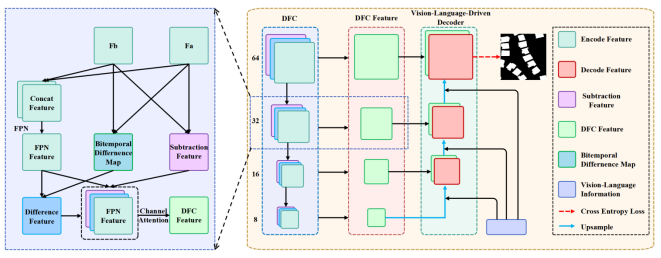
\includegraphics[width=\textwidth]{paper_figures/基于AI基础模型微调的变化检测模型研究/ChangeCLIP/changeclip4.png}
  \caption{ChangeCLIP 的差分特征补偿模块和解码结构。Concat Feature 指的是在编码阶段通过将双时相图像拼接而获得的特征图。Bitemporal Difference Map 指的是通过计算余弦相似度得到的差异图。Subtraction Feature 指的是将双时相图像的特征图相减而得到的特征。}
  \label{fig:changeclip4}
\end{figure}

为了增强 ChangeCLIP 在解码阶段的学习能力,基于 Swin Transformer 块设计了逐层的多级特征融合结构。该结构将高层特征信息传递至低层,并在每个融合级别使用 Swin Transformer 块提升解码表征能力。如图~\ref{fig:changeclip4}所示,详细介绍了 ChangeCLIP 的视觉–语言驱动解码器。在编码阶段,ChangeCLIP 将文本语义信息与图像特征图融合;在解码阶段,对双时相遥感影像的不同特征应用多级特征融合的多模态解码模块,最终获得解码预测结果。其计算步骤如下:
\begin{align}
F_3 &= \mathrm{concat}\bigl(f(D_4,\;\text{text}),\;D_3\bigr)\, \label{eq:changeclip-23}\\
F_2 &= \mathrm{concat}\bigl(f(F_3,\;\text{text}),\;D_2\bigr)\, \label{eq:changeclip-24}\\
F_1 &= \mathrm{concat}\bigl(f(F_2,\;\text{text}),\;D_1\bigr)\, \label{eq:changeclip-25}\\
\mathrm{output} &= \mathrm{Upsample}(F_1)\, \label{eq:changeclip-26}
\end{align}
其中,$D_1, D_2, D_3, D_4$ 是由 DFC 模块生成的不同特征图,$\text{text}$ 是编码阶段提取的双时相视觉–语言特征序列;$f$ 表示 Swin Transformer 块,$\mathrm{output}$ 是通过上采样操作得到的最终预测结果。

总而言之,本节提出了一种强大的视觉-语言驱动解码器,应用于遥感影像变化检测(RSCD)任务中。视觉-语言驱动解码器利用Swin Transformer模块建立全局注意力关系,从而能够在不同层级上对差异特征图进行优化解码,增强了模型在解码阶段的特征表示能力。为了进一步增强解码阶段的表现,引入了一个低秩双线性注意力模块。该模块有效地将编码阶段的视觉-语言特征与解码阶段的视觉特征结合,通过补充解码阶段的语义特征,使得模型能够从遥感影像中提取重要的变化特征,从而实现更精确的变化检测。最后,设计了一个逐层结构来构建解码模块。基于Swin Transformer模块的逐层特征融合结构确保了特征信息从高层到低层的传递,从而保证了在解码阶段能够全面利用重要特征,提升了遥感影像变化检测的性能。总体而言,ChangeCLIP在RSCD任务中利用了视觉-语言驱动的解码器。通过有效地整合视觉和文本信息,实现了对遥感影像变化的更好理解和检测。

\subsection{实验结果与分析}

\begin{figure}[!htbp]
  \centering
  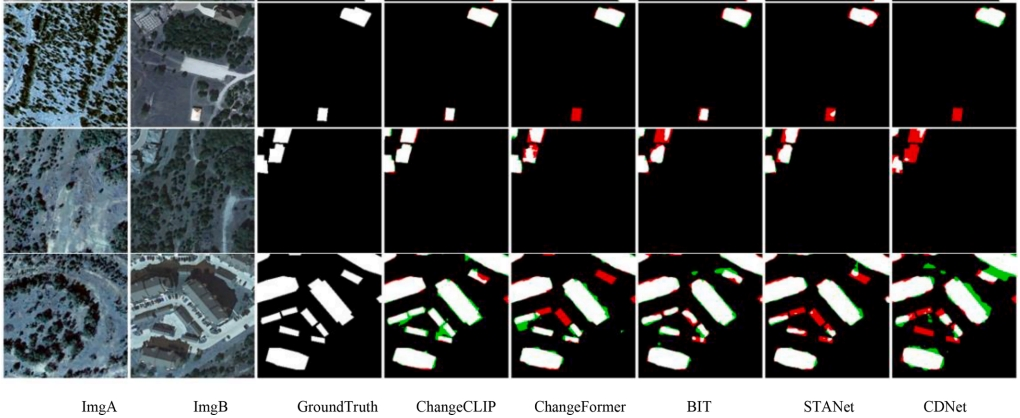
\includegraphics[width=\textwidth]{paper_figures/基于AI基础模型微调的变化检测模型研究/ChangeCLIP/changeclip_levir.png}
  \caption{ChangeCLIP 模型与对比模型在 LEVIR-CD 上的局部可视化对比结果}
  \label{fig:changeclip_levir}
\end{figure}

与之相比,ChangeCLIP首创了一种专门针对遥感变化检测(RSCD)的创新多模态视觉-语言框架,巧妙地融合了视觉和文本数据。通过引入独特的模块,如差异特征补偿(DFC)模块和视觉-语言驱动解码器,进一步创新。这些组件协同作用,增强了变化相关特征的学习和语义理解。多模态输入、差异特征学习和视觉-语言综合的结合使得ChangeCLIP在多个数据集上达到了新的性能基准,取得了最先进的结果。对比分析实验证实了ChangeCLIP在执行RSCD任务时,在CNN、注意力、Transformer、特征融合/差异化和边界感知等多个类别的现有模型中的优越性。

\subsubsection{实验结果量化指标与可视化分析}

如表~\ref{tab:changeclip_levir}、表~\ref{tab:changeclip_levirplus}、表~\ref{tab:changeclip_whucd}、表~\ref{tab:changeclip_cdd}至表~\ref{tab:changeclip_sysu}所示,在五个数据集(LEVIR-CD、LEVIR-CD+、WHUCD、CDD和SYSU-CD)上广泛评估了ChangeCLIP。根据各种评估指标,ChangeCLIP在所有数据集上都达到了最先进的性能。符号``--''表示原始论文中缺失的数据。对于这些情况,重新训练了部分模型,以获得更高的准确性。与其他变化检测方法相比,ChangeCLIP算法在多种评估指标上表现出了优越的性能。由于这些是二分类变化检测任务,前景变化类别的交并比(IoU)作为主要指标。

对实验结果进行仔细分析发现,在LEVIR-CD数据集上,ChangeCLIP在所有指标上超越了最近的经典变化检测算法。特别是,RN50主干网络达到了85.20\%的IoU。在LEVIR-CD+数据集上,ChangeCLIP在所有标准上都领先于其他方法,且优势显著。此外,ViT主干网络的IoU达到了75.63\%,超过了RN50主干网络。在WHUCD数据集上,ViT和RN50主干网络的IoU均超过了90\%。在这三个以建筑物为重点的数据集中,ChangeCLIP在处理密集小物体场景方面展现出了强大的有效性。ChangeCLIP在LEVIR-CD、LEVIR-CD+和WHUCD上的召回率分别为90.67\%、83.90\%和94.02\%,表明其具有较高的真正检测率和较低的假阴性发生率。这表明ChangeCLIP在实际应用中具有显著的实用价值。

\begin{figure}[!htbp]
  \centering
  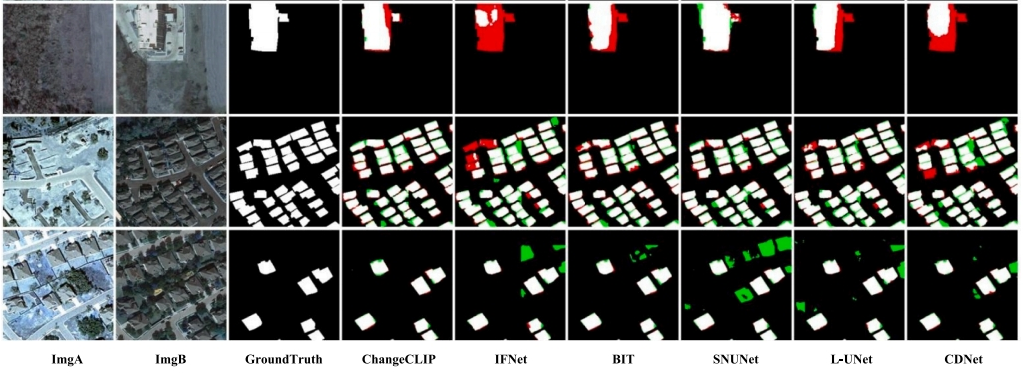
\includegraphics[width=\textwidth]{paper_figures/基于AI基础模型微调的变化检测模型研究/ChangeCLIP/changeclip_levirplus.png}
  \caption{ChangeCLIP 模型与对比模型在 LEVIR-CD+ 上的局部可视化对比结果}
  \label{fig:changeclip_levirplus}
\end{figure}

在CDD数据集上,ChangeCLIP达到了95.87\%的IoU,超过了最近提出的变化检测算法。这一表现展示了ChangeCLIP在检测一般变化区域方面的能力,同时也证明了CDD数据集高质量的标注,使得ChangeCLIP强大的拟合能力得以充分发挥。在SYSU-CD数据集上,ChangeCLIP达到了71.41\%的IoU,同样超越了最新的算法。与CDD类似,SYSU-CD也是为检测一般变化区域而设计的。

在图~\ref{fig:changeclip_levir}、图~\ref{fig:changeclip_levirplus}、图~\ref{fig:changeclip_whucd}、图~\ref{fig:changeclip_cdd}和图~\ref{fig:changeclip_sysu}中,展示了在LEVIR-CD、LEVIR-CD+、WHUCD、CDD和SYSU-CD上的测试结果可视化。选择了ChangeCLIP模型中IoU得分最高的模型,并将其与近年来的经典算法进行比较。在这些可视化结果中,真正阳性(TP)由白色像素表示,真正阴性(TN)由黑色表示,假阳性(FP)由绿色表示,假阴性(FN)由红色表示。可视化结果明确展示了ChangeCLIP在各种数据集和应用场景中都能实现出色的检测性能,与地面真实标注紧密对齐。

\begin{table}[!htbp]
  \centering
  \caption{ChangeCLIP 模型在 LEVIR-CD 数据集上的定量结果}
  \label{tab:changeclip_levir}
  \begin{tabular*}{\textwidth}{@{\extracolsep{\fill}} l c c c c c c c}
    \toprule
    Model & OA & mF1 & mIoU & IoU & F1 & Rec & Prec \\
    \midrule
    CDNet~\cite{Alcantarilla2016StreetviewCD}                         & 98.35 & 91.49 & 85.25 & 72.21 & 83.87 & 84.14 & 83.61 \\
    STANet~\cite{chen_spatial-temporal_2020}                        & 98.92 & 94.22 & 89.54 & 80.20 & 89.02 & 85.80 & 92.49 \\
    BIT~\cite{chen_remote_2022}                           & 98.95 & 93.22 & 89.93 & 80.86 & 89.48 & 87.53 & 90.65 \\
    MFATNet~\cite{Mao2022MFATNetMF}                       & 99.03 & --    & --    & 82.42 & 90.36 & 88.93 & 91.85 \\
    ChangeFormer~\cite{bandara2022transformer}                  & 99.04 & --    & 90.82 & 82.66 & 90.50 & 90.18 & 90.83 \\
    HMCNet~\cite{Wang2022HMCNetHE}                        & 99.07 & --    & --    & 83.05 & 90.74 & 89.82 & 91.68 \\
    AFCF3D-Net~\cite{Ye2023AdjacentLevelFC}                    & --    & --    & --    & 83.08 & 90.76 & 90.17 & 91.35 \\
    LGPNet~\cite{Liu2022BuildingCD}                        & 99.16 & --    & 91.38 & 83.63 & 91.09 & 89.38 & 92.87 \\
    TransUNetCD~\cite{Li2022TransUNetCDAH}                   & --    & --    & --    & 83.67 & 91.11 & 89.82 & 92.43 \\
    FHD~\cite{pei_feature_2022}                           & 99.10 & 95.33 & 91.39 & 83.72 & 91.14 & 90.32 & 91.97 \\
    DMATNet~\cite{Song2022RemoteSI}                       & 98.25 & --    & --    & 84.13 & 90.75 & 89.98 & 91.56 \\
    STransUNet~\cite{Yuan2022STransUNetAS}                    & 99.13 & --    & --    & 84.19 & 91.41 & 90.55 & 92.30 \\
    \textbf{ChangeCLIP (RN50)}    & \textbf{99.20} & \textbf{95.79} & \textbf{92.18} & \textbf{85.20} & \textbf{92.01} & \textbf{90.67} & \textbf{93.40} \\
    ChangeCLIP (ViT-B/16)         & 99.14 & 95.42 & 91.54 & 83.99 & 91.30 & 89.04 & 93.68 \\
    \bottomrule
  \end{tabular*}
\end{table}

\begin{table}[!htbp]
  \centering
  \caption{ChangeCLIP 模型在 LEVIR-CD+ 数据集上的定量结果}
  \label{tab:changeclip_levirplus}
  \begin{tabular*}{\textwidth}{@{\extracolsep{\fill}} l c c c c c}
    \toprule
    Model & OA & IoU & F1 & Rec & Prec \\
    \midrule
    FC-Siam-Di~\cite{Daudt2018FullyCS}               & 98.14 & 61.37 & 76.06 & 72.55 & 79.94 \\
    CDNet~\cite{Alcantarilla2016StreetviewCD}                    & 98.01 & 61.58 & 76.22 & 78.45 & 74.12 \\
    FresUNet~\cite{Daudt2018MultitaskLF}                 & 98.28 & 65.24 & 78.96 & 79.30 & 78.62 \\
    L-UNet~\cite{Papadomanolaki2021ADM}                   & 98.36 & 67.19 & 80.38 & 82.25 & 78.59 \\
    SNUNet~\cite{Fang2021SNUNetCDAD}                   & 98.42 & 68.17 & 80.82 & 79.43 & 80.52 \\
    DTCDSCN~\cite{Liu2019BuildingCD}                  & 98.58 & 68.76 & 81.19 & 79.08 & 83.41 \\
    BIT~\cite{chen_remote_2022}                      & 98.49 & 69.07 & 81.71 & 82.84 & 80.61 \\
    DSIFN~\cite{Zhang2020ADS}                    & 98.61 & 70.97 & 82.29 & 80.32 & 83.77 \\
    ICIF-Net~\cite{Feng2022ICIFNetIC}                 & 98.73 & 71.89 & 83.65 & 80.88 & 87.79 \\
    ChangeCLIP (RN50)        & 98.79 & 73.61 & 84.80 & 82.69 & 87.02 \\
    \textbf{ChangeCLIP (ViT-B/16)} & \textbf{98.90} & \textbf{75.63} & \textbf{86.12} & \textbf{83.90} & \textbf{88.46} \\
    \bottomrule
  \end{tabular*}
\end{table}

\begin{table}[!htb]
  \centering
  \caption{ChangeCLIP 模型在 WHUCD 数据集上的定量结果}
  \label{tab:changeclip_whucd}
  \begin{tabular}{@{}lccccccc@{}}
    \toprule
    Model                      & OA    & mF1   & mIoU  & IoU   & F1    & Rec   & Prec   \\
    \midrule
    DPCCNet~\cite{Papadomanolaki2021ADM}                    & 98.27 & 90.42 & 83.67 & 69.13 & 81.75 & 83.77 & 79.83  \\
    SNUNet~\cite{Fang2021SNUNetCDAD}                     & 98.22 & 90.92 & 84.38 & 70.61 & 82.77 & 92.31 & 75.03  \\
    BIT~\cite{chen_remote_2022}                        & 98.62 & 90.50 & 86.78 & 75.00 & 85.71 & 89.74 & 82.04  \\
    DARNet~\cite{li_densely_2022}                     & 98.75 & 93.14 & 87.79 & 76.89 & 86.93 & 89.85 & 84.20  \\
    ICIFNet~\cite{Feng2022ICIFNetIC}                    & 99.01 & 94.32 & 89.70 & 80.43 & 89.16 & 87.58 & 90.79  \\
    DSIFN~\cite{Zhang2020ADS}                      & 99.14 & 94.94 & 90.74 & 82.37 & 90.33 & 87.13 & 93.78  \\
    P2V~\cite{lin_transition_2023}                        & 99.32 & 96.08 & 92.68 & 86.07 & 92.52 & 90.91 & 94.18  \\
    ChangeCLIP (RN50)          & 99.52 & 97.29 & 94.83 & 90.15 & 94.82 & 94.02 & 95.63  \\
    ChangeCLIP (ViT-B/16)      & 99.52 & 97.27 & 94.79 & 90.08 & 94.78 & 93.58 & 96.02  \\
    \bottomrule
  \end{tabular}
\end{table}

\begin{table}[!htb]
  \centering
  \caption{ChangeCLIP 模型在 CDD 数据集上的定量结果}
  \label{tab:changeclip_cdd}
  \begin{tabular*}{\textwidth}{@{\extracolsep{\fill}} l c c c c c c c}
    \toprule
    Model & OA & mF1 & mIoU & IoU & F1 & Rec & Prec \\
    \midrule
    DSAMNet~\cite{shi_deeply_2022}                 & --    & --    & --    & 88.13 & 93.69 & 92.77 & 94.54 \\
    BESNet~\cite{Lei2022BoundaryEC}                  & 98.51 & --    & 93.30 & 88.28 & 93.77 & 92.39 & 95.20 \\
    SwinSUNet~\cite{zhang_swinsunet_2022}               & 98.50 & --    & --    & --    & 94.00 & 92.30 & 95.70 \\
    ISNet~\cite{Cheng2022ISNetTI}                   & 98.78 & 97.06 & 94.37 & 90.12 & 94.80 & 94.43 & 95.18 \\
    D-TNet~\cite{wan_d-tnet_2022-3}                  & 98.90 & --    & --    & 91.18 & 95.39 & 96.75 & 94.06 \\
    JFSDNet~\cite{Zhou2022JointFD}                 & 99.07 & --    & --    & --    & 95.55 & 92.60 & \textbf{98.75} \\
    IRA-MRSNet~\cite{Ling2022IRAMRSNetAN}              & 99.14 & --    & --    & --    & 96.47 & 96.13 & 96.81 \\
    RCDT~\cite{Lu2022RCDTRR}                    & --    & --    & --    & 93.79 & 96.80 & 96.97 & 96.63 \\
    SSANet~\cite{Jiang2022JointVL}                  & --    & --    & --    & 95.20 & 94.33 & 96.06 & \textbf{99.07} \\
    \textbf{ChangeCLIP (RN50)}    & \textbf{99.48} & \textbf{98.80} & \textbf{97.64} & \textbf{95.87} & \textbf{97.89} & 97.77 & 98.02 \\
    ChangeCLIP (ViT-B/16)   & 99.47 & 98.77 & 97.59 & 95.78 & 97.85 & \textbf{97.81} & 97.88 \\
    \bottomrule
  \end{tabular*}
\end{table}

\begin{table}[!htb]
  \centering
  \caption{ChangeCLIP 模型在SYSU-CD数据集上的定量结果}
  \label{tab:changeclip_sysu}
  \begin{tabular*}{\textwidth}{@{\extracolsep{\fill}} l c c c c c c c}
    \toprule
    Model & OA & mF1 & mIoU & IoU & F1 & Rec & Prec \\
    \midrule
    DSAMNet~\cite{shi_deeply_2022}                   & --    & --    & --    & 64.18 & 78.18 & \textbf{81.86} & 74.81 \\
    CDNet~\cite{Alcantarilla2016StreetviewCD}                     & 89.90 & 85.86 & 75.99 & 64.34 & 78.30 & 77.29 & 79.34 \\
    ISNet~\cite{Cheng2022ISNetTI}                     & 90.01 & --    & --    & 64.44 & 78.29 & 80.27 & 76.41 \\
    SNUNet~\cite{Fang2021SNUNetCDAD}                    & 90.79 & 86.80 & 77.41 & 66.02 & 79.54 & 75.87 & 83.58 \\
    L-UNet~\cite{Papadomanolaki2021ADM}                    & 90.58 & 86.75 & 77.30 & 66.15 & 79.63 & 78.08 & 81.24 \\
    DSIFN~\cite{Zhang2020ADS}                       & 90.74 & 87.06 & 77.75 & 66.90 & 80.17 & 79.37 & 80.98 \\
    DPCC-Net~\cite{Papadomanolaki2021ADM}                  & --    & --    & --    & 66.63 & 79.97 & 78.93 & 81.05 \\
    DARNet~\cite{li_densely_2022}                    & 91.26 & --    & --    & 68.10 & 81.03 & 79.11 & 83.04 \\
    ICIFNet~\cite{Feng2022ICIFNetIC}                   & 91.24 & --    & --    & 68.12 & 80.74 & 78.51 & 83.37 \\
    SSANet~\cite{Jiang2022JointVL}                    & --    & --    & --    & 68.18 & 81.08 & 79.73 & 82.48 \\
    ChangeCLIP (RN50)         & 92.08 & 88.79 & 80.38 & 70.53 & 82.72 & 80.41 & 85.16 \\
    AFCF3D-Net~\cite{Ye2023AdjacentLevelFC}                & --    & --    & --    & 71.09 & 83.11 & \textbf{83.88} & 82.30 \\
    \textbf{ChangeCLIP (ViT-B/16)} & \textbf{92.46} & \textbf{89.23} & \textbf{81.06} & \textbf{71.41} & \textbf{83.32} & 79.80 & \textbf{87.16} \\
    \bottomrule
  \end{tabular*}
\end{table}

\begin{figure}[!htbp]
  \centering
  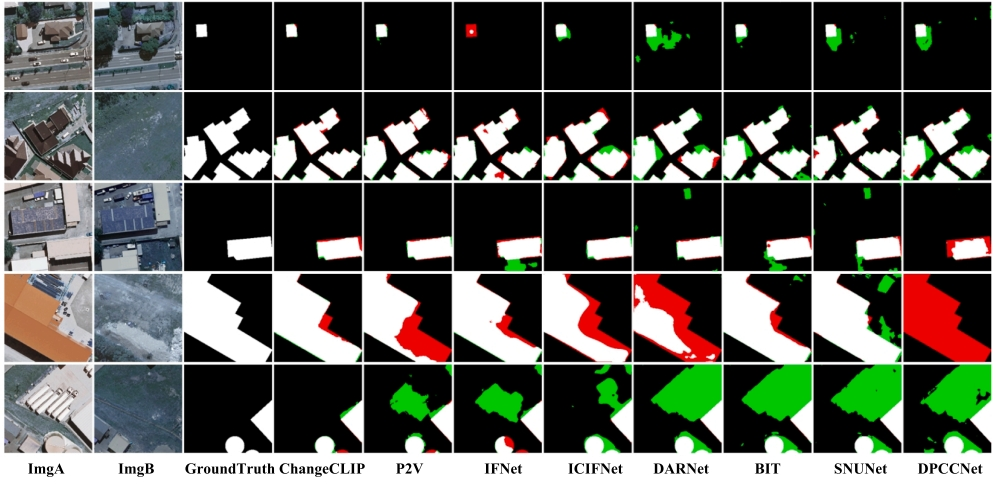
\includegraphics[width=\textwidth]{paper_figures/基于AI基础模型微调的变化检测模型研究/ChangeCLIP/changeclip_whucd.png}
  \caption{ChangeCLIP 模型与对比模型在WHUCD数据集上的可视化对比结果}
  \label{fig:changeclip_whucd}
\end{figure}

% \begin{comment}

\subsubsection{ChangeCLIP消融实验}

如表~\ref{tab:changeclip_ablation_resnet}和表~\ref{tab:changeclip_ablation_vit}所示,进行了广泛的消融实验,以验证ChangeCLIP中关键组件的贡献,包括多模态编码器(ME)、差异特征补偿(DFC)模块和视觉-语言驱动解码器(VLDD)。由于变化检测任务中前景类和背景类的比例差异很大,表VIII使用前景类的IoU指数作为比较的基础。基线模型仅使用CLIP的主干网络作为图像编码器,并使用基础的FPN结构进行双时相特征融合。基线模型中的解码器是FCN。该单模态模型提供了性能基准。逐步添加ME、DFC和VLDD模块在各数据集上持续提高准确性,证明了每个创新的价值。ME指的是使用图像和文本信息的多模态编码器,DFC表示加入差异特征补偿模块,VLDD表示视觉-语言驱动解码器。

在消融实验的三个实验中比较了变化检测任务中常用的差异特征计算模块,包括Concat、减法和DFC模块。该部分的消融实验结果表明,直接使用减法进行差异特征计算的表现不如使用Concat进行双时相特征融合。这与前文的分析一致。与Concat相比,DFC模块通过结合不同方面的差异特征,具有更强的差异特征表示能力。

\begin{figure}[!htbp]
  \centering
  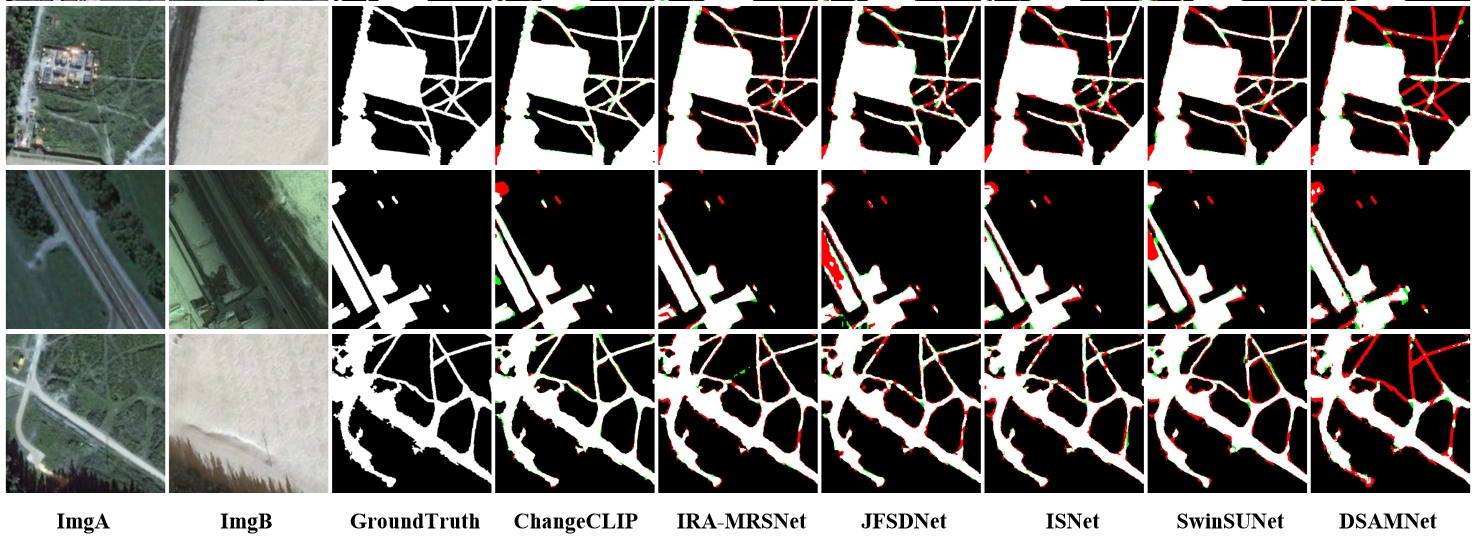
\includegraphics[width=\textwidth]{paper_figures/基于AI基础模型微调的变化检测模型研究/ChangeCLIP/changeclip_cdd.png}
  \caption{ChangeCLIP 模型与对比模型在 CDD 上的可视化对比结果}
  \label{fig:changeclip_cdd}
\end{figure}

\begin{figure}[!htbp]
  \centering
  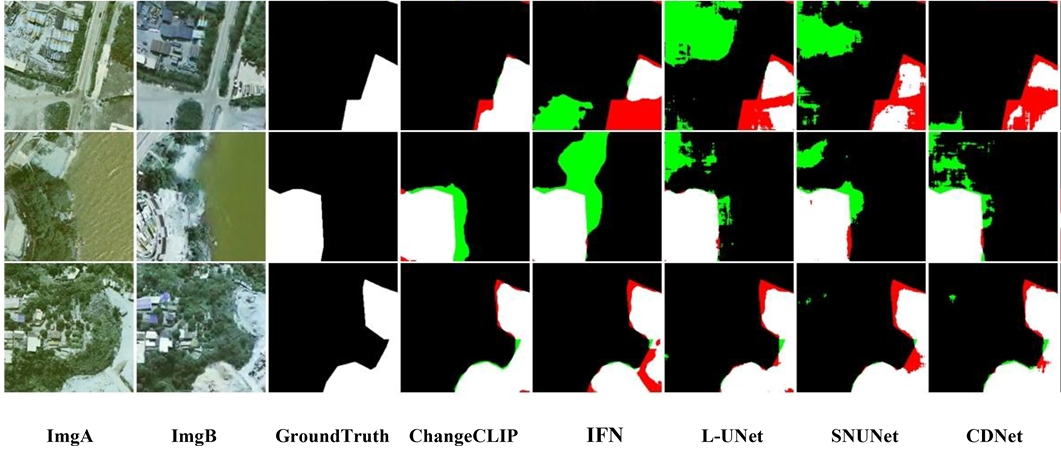
\includegraphics[width=\textwidth]{paper_figures/基于AI基础模型微调的变化检测模型研究/ChangeCLIP/changeclip_sysu.png}
  \caption{ChangeCLIP 模型与对比模型在 SYSU-CD 上的可视化对比结果}
  \label{fig:changeclip_sysu}
\end{figure}

\begin{figure}[!htbp]
  \centering
  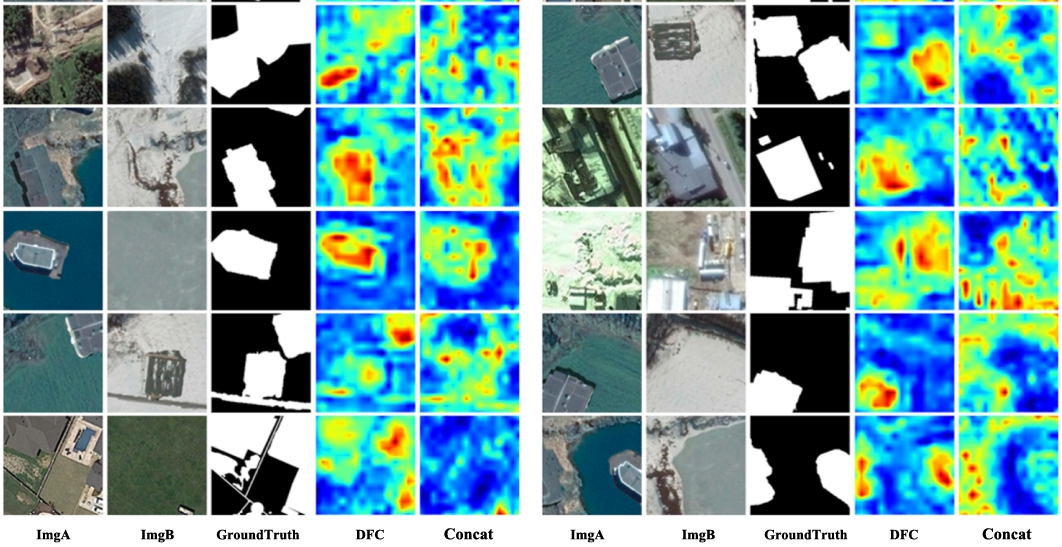
\includegraphics[width=\textwidth]{paper_figures/基于AI基础模型微调的变化检测模型研究/ChangeCLIP/changeclip_hotmap.png}
  \caption{不同的差异特征方法与 ChangeCLIP 的特征热图在 CDD 数据集上的可视化对比结果}
  \label{fig:changeclip_hotmap}
\end{figure}

具体来说,通过ME集成文本语义与基于视觉的基线相比,性能有所提升,突出了多模态的优势。显然,通过多模态信息补充图像信息,有助于增强模型对遥感图像中语义特征的理解。由于VLDD需要包括来自ME组件的视觉-语言信息,无法仅对Baseline+VLDD进行消融研究。因此,将Baseline+ME和Baseline+ME+VLDD的实验结果进行了比较。可以看出,VLDD在解码器中结合了文本和视觉表示,带来了额外的提升。

\begin{table}[!htb]
\centering
\small
\setlength{\tabcolsep}{2pt} % 紧凑列距
\caption{基于 RN50 骨干的 IoU 消融实验。Base:仅用图像编码器;ME:多模态编码器;I:Image Encoder;T:Text Encoder;DFC:差异特征补偿;VLDD:视觉-语言驱动解码器;FPN:特征金字塔;FCN:全卷积;Sub:减法。}
\label{tab:changeclip_ablation_resnet}
\begin{tabular}{@{}l c c c *{5}{c}@{}}
\toprule
\textbf{Model} & \textbf{Encoder} & \textbf{Neck} & \textbf{Decoder} &
\makecell{\textbf{LEVIR-}\\\textbf{CD}} &
\makecell{\textbf{LEVIR-}\\\textbf{CD+}} &
\textbf{CDD} &
\makecell{\textbf{SYSU-}\\\textbf{CD}} &
\textbf{WHU} \\
\midrule
Base            & I     & FPN       & FCN  & 75.25 & 68.61 & 89.74 & 61.71 & 87.56 \\
Base(Sub)       & I     & FPN(Sub)  & FCN  & 71.19 & 60.98 & 86.37 & 44.13 & 80.88 \\
Base+DFC        & I     & FPN+DFC   & FCN  & 75.85 & 70.46 & 89.86 & 69.34 & 89.01 \\
Base+ME         & I\&T  & FPN       & FCN  & 76.01 & 70.51 & 89.91 & 65.64 & 87.74 \\
Base+ME+VLDD    & I\&T  & FPN       & VLDD & 84.72 & 72.62 & 95.72 & 68.68 & 89.59 \\
ChangeCLIP      & I\&T  & FPN+DFC   & VLDD & 85.20 & 73.61 & 95.87 & 70.53 & 90.15 \\
\bottomrule
\end{tabular}
\end{table}


\begin{table}[!htb]
\centering
\small
\setlength{\tabcolsep}{2pt}
\caption{基于 ViT-B/16 骨干的 IoU 消融实验。记号同表 \ref{tab:changeclip_ablation_resnet}。}
\label{tab:changeclip_ablation_vit}
\begin{tabular}{@{}l c c c *{5}{c}@{}}
\toprule
\textbf{Model} & \textbf{Encoder} & \textbf{Neck} & \textbf{Decoder} &
\makecell{\textbf{LEVIR-}\\\textbf{CD}} &
\makecell{\textbf{LEVIR-}\\\textbf{CD+}} &
\textbf{CDD} &
\makecell{\textbf{SYSU-}\\\textbf{CD}} &
\textbf{WHU} \\
\midrule
Base            & I     & FPN       & FCN  & 74.73 & 68.16 & 88.77 & 64.82 & 79.22 \\
Base(Sub)       & I     & FPN(Sub)  & FCN  & 74.31 & 68.75 & 83.67 & 64.45 & 79.73 \\
Base+DFC        & I     & FPN+DFC   & FCN  & 75.24 & 68.59 & 90.25 & 68.42 & 82.53 \\
Base+ME         & I\&T  & FPN       & FCN  & 75.35 & 69.12 & 90.54 & 65.64 & 82.83 \\
Base+ME+VLDD    & I\&T  & FPN       & VLDD & 83.41 & 71.73 & 94.13 & 69.76 & 82.81 \\
ChangeCLIP      & I\&T  & FPN+DFC   & VLDD & 83.99 & 75.63 & 95.78 & 71.41 & 90.08 \\
\bottomrule
\end{tabular}
\end{table}




有趣的是,DFC本身的表现几乎与ME相同,这表明在ChangeCLIP中,变化特征建模和多模态信息对变化检测任务的影响是相等的。将减法作为双时相图像融合方法在FPN之前的效果比Concat更差。这可能是因为直接使用特征减法会丢失大部分双时相图像的信息,使得网络难以学习变化的表示。包含所有组件的完整ChangeCLIP模型达到了最佳结果,每个模块提供了互补的优势。总之,广泛消融分析定量展示了ChangeCLIP中提出的多模态编码器、差异特征补偿模块和视觉-语言驱动解码器的独特贡献。通过与消融版本和基线模型的准确性提升,验证了ChangeCLIP 模型中的创新。

\begin{table}[!htb]
  \centering
  \caption{ChangeCLIP模型在RSCD数据集上基于ResNet-50和ViT-B/16骨干模型的结果}
  \label{tab:changeclip_backbone}
  \begin{tabular*}{\textwidth}{@{\extracolsep{\fill}} l l c c c c c c c}
    \toprule
    Dataset       & Backbone     & OA    & mF1   & mIoU  & IoU   & F1    & Rec   & Prec  \\
    \midrule
    \multirow{2}{*}{WHUCD}
                  & RN50         & 99.52 & 97.29 & 94.83 & 90.15 & 94.82 & 94.02 & 95.63 \\
                  & ViT-B/16     & 99.52 & 97.27 & 94.79 & 90.08 & 94.78 & 93.58 & 96.02 \\
    \midrule
    \multirow{2}{*}{CDD}
                  & RN50         & 99.48 & 98.80 & 97.64 & 95.87 & 97.89 & 97.77 & 98.02 \\
                  & ViT-B/16     & 99.47 & 98.77 & 97.59 & 95.78 & 97.85 & 97.81 & 97.88 \\
    \midrule
    \multirow{2}{*}{SYSU-CD}
                  & RN50         & 92.08 & 88.79 & 80.38 & 70.53 & 82.72 & 80.41 & 85.16 \\
                  & ViT-B/16     & 92.46 & 89.23 & 81.06 & 71.41 & 83.32 & 79.80 & 87.16 \\
    \midrule
    \multirow{2}{*}{LEVIR-CD}
                  & RN50         & 99.20 & 95.79 & 92.18 & 85.20 & 92.01 & 90.67 & 93.40 \\
                  & ViT-B/16     & 99.14 & 95.42 & 91.54 & 83.99 & 91.30 & 89.04 & 93.68 \\
    \midrule
    \multirow{2}{*}{LEVIR-CD+}
                  & RN50         & 98.79 & 92.08 & 86.18 & 73.61 & 84.80 & 82.69 & 87.02 \\
                  & ViT-B/16     & 98.90 & 92.77 & 87.24 & 75.63 & 86.12 & 83.90 & 88.46 \\
    \bottomrule
  \end{tabular*}
\end{table}



\subsubsection{ChangeCLIP在不同的骨架网络的结果}

根据本节的实验,对CLIP模型中的两个骨干网络,RN50(ResNet50)和ViT(ViT-B/16),进行了详细比较。根据表表~\ref{tab:changeclip_backbone}中的结果,在使用的5个代表性数据集上,ViT骨干网络在SYSU-CD和LEVIR-CD+数据集上的表现远优于RN50骨干网络,在CDD和WHUCD数据集上接近RN50,在LEVIR-CD数据集上的表现则较差。可以看出,ViT和RN50在不同数据集上的表现有所不同,但总体上它们都表现出了较高的准确性。ViT的整体表现略优于RN50。这可以归因于几个因素。首先,ViT相比RN50模型具有更广泛的全局感受野。这意味着ViT能够更好地捕捉遥感影像中目标个体之间的全局关联信息。其次,在RN50骨干网络中,使用了一个注意力池化模块来生成高层语义特征,这些特征被用来替代图像序列特征。而在ViT框架中,直接将高层特征作为图像序列特征。与RN50骨干网络相比,ViT骨干网络生成的图像序列特征与文本序列特征更加一致,这使得ViT骨干网络在多模态任务中表现得更好。

\subsubsection{ChangeCLIP中差异特征图热图可视化分析}

可视化热图为ChangeCLIP在遥感影像变化检测(RSCD)任务中感知变化特征的能力提供了宝贵的见解。观察可得,使用ChangeCLIP能够生成具有更强判别性的特征图,这表明其对遥感影像中变化区域的敏感度增强。与传统的特征图热图通常突出前景中的显著区域不同,变化检测的主要目标是识别变化区域。在图~\ref{fig:changeclip_hotmap}中,展示了ChangeCLIP在CDD数据集上的特征图可视化。具体而言,``DFC''表示通过DFC模块处理后的融合特征图的编码部分特征,而``Concat''表示双时相影像在图像特征提取后得到的融合特征图。从图中可以看出,与DFC模块之前的特征图相比,经过DFC模块处理后的特征图在变化特征上展现了更好的效果。特征热图展示了ChangeCLIP在双时相遥感影像中对变化区域的强烈感知能力,突显了本节提出的方法在变化检测任务中的优越性。

\subsection{ChangeCLIP模型的可行性分析与未来工作展望}

\subsubsection{基于多模态视觉-语言表示学习的变化检测}

在本节中,结合了CLIP的无监督推理能力,为遥感影像构建了基本的文本提示。然而,类别语义信息通常在遥感影像语义分割中更为重要,因为在变化检测中,目标是感知变化区域,而不是区分特定的类别。因此,在变化检测任务中指定文本提示需要更好地契合变化检测的任务需求。因此,背景类别很难为变化检测任务制定合适的文本提示。根据提出的消融实验,显然,结合文本的多模态变化检测在多个数据集上始终能达到卓越的算法精度。可以明确看出,多模态信息的融合确实为推动遥感影像变化检测(RSCD)在不同数据集上的进展做出了贡献。同时,在提出的方法的解码阶段,引入了一种新机制,进一步增强了变化检测的性能。通过引入低秩双线性注意力模块,促进了来自解码阶段的图像特征与编码阶段的视觉-语言特征的融合。这种集成使得模型能够有效捕捉视觉和文本模态之间的互补信息,从而提升特征表示和增强RSCD性能。低秩双线性注意力机制促进了解码特征与编码的视觉-语言特征的对齐和交互,增强了模型捕捉遥感影像语义上下文的能力。这种创新的融合方法加强了模型对RSCD任务的理解,并提高了其在遥感影像变化识别中的判别能力。然而,针对解码阶段的视觉-语言结合,可以探索一种更合适的方式,将编码阶段的视觉-语言特征与解码阶段的视觉特征进行结合。

\subsubsection{image-score map的应用}

在本节提出的ChangeCLIP中,基于文本提示和图像视觉信息计算了图像-文本得分图。对于图像-文本得分图的应用,将得分图与视觉编码阶段的高层语义特征图进行拼接,并直接利用文本信息来补充语义信息。依据在语义分割任务中广泛应用的多层次特征融合理论,得分图可以与高层语义特征图及浅层特征图进行结合,以在浅层网络阶段补充文本的语义信息。然而,在实际的网络设计中,生成多层次的得分图需要大量的计算。因此,在结合得分图与视觉编码阶段的过程中,仍有很大的改进空间,可以构思出一个合适的模块来更好地将得分图与视觉编码阶段结合。

\subsubsection{差异特征计算}

在标准变化检测模型中,依赖语义分割任务是常见的做法。然而,在变化检测任务中,重点应该是提取和学习目标区域的变化特征。基于常用的差异特征计算方法,设计了一个差异特征补偿(DFC)模块。DFC模块整合了几种常用的差异特征构建方法,使网络能够以自适应的方式有效学习来自不同差异特征构建方法的差异特征。通过增强变化检测网络学习变化特征的能力,DFC模块有效提升了ChangeCLIP的性能。

在不同数据集上的实验结果揭示了提高变化检测准确性的两种主要方式。首先,像Transformer这样的强大特征提取器可以增强网络对遥感影像的表示能力。其次,像特征融合和差异化这样的技术可以帮助网络更好地捕捉变化特征。在LEVIR-CD+和CDD等数据集上的结果显著提高了网络的性能,其中ChangeCLIP利用Transformer和DFC模块取得了最先进的结果。因此,未来应该更多关注变化相关特征的学习,使得网络更符合变化的识别,从而提高变化检测算法的效果。

\subsection{小结}

在本节中,提出了一种名为ChangeCLIP的多模态框架,用于通过利用多模态视觉-语言信息在遥感影像中进行变化检测。通过整合遥感影像的文本语义信息,增强了视觉模型感知遥感变化的能力。提出的差异特征补偿模块整合了常用的差异特征计算方法,优化了变化检测中差异特征融合的方式。此外,还提出了一种名为视觉-语言驱动解码器的多模态变化检测解码方法,旨在补充解码阶段的语义信息。在解码阶段融合文本和视觉特征,使得ChangeCLIP能够生成更准确和全面的表示,提升变化检测任务的性能。为了评估ChangeCLIP的有效性,在5个基准变化检测数据集(LEVIR-CD、LEVIR-CD+、WHUCD、CDD和SYSU-CD)上进行了全面的实验。实验结果表明,提出的ChangeCLIP模型显著优于现有的最先进方法,在所有5个数据集上达到了前所未有的性能。此外,本节还对ChangeCLIP进行了系统分析,揭示了其潜在的机制,并为未来可能的改进提供了见解。展望未来,多模态范式将在遥感图像处理领域获得越来越多的关注。通过开发更有效的变化检测语言提示,ChangeCLIP的性能有着巨大的提升空间,同时,ChangeCLIP也将成为多模态遥感影像变化检测(RSCD)的基准。这些合适的提示可以更好地引导模型学习与变化相关的特征,进而进一步提高变化检测性能。


\section{基于视觉基础模型微调的变化检测方法}

\subsection{视觉基础模型与变化检测任务概述}

遥感影像变化检测(Remote Sensing Change Detection, RSCD)是遥感领域的重要研究方向,其目标是通过对比多时相遥感影像来识别地表的变化区域。在实际应用中,RSCD 面临多重挑战。首先,遥感数据具有多时相性、多源多样性和多尺度变化等特征。其次,现有高分辨率遥感数据集往往规模有限,标注成本高昂,且缺乏充足的大规模预训练样本。此外,由于异构传感器和成像条件变化所导致的域偏移问题,严重阻碍了现有模型的跨域泛化能力。这些问题在复杂场景下会导致变化检测模型性能的下降。

近年来,深度学习的快速发展不断推动着变化检测方法的演进。从早期的卷积神经网络(CNNs)到视觉 Transformer,再到近期的通用视觉基础模型(Vision Foundation Models, VFMs),模型的特征提取与泛化能力逐步增强。VFMs 如 SAM~\cite{Kirillov2023SegmentA}、DINO~\cite{Caron2021EmergingPI,simeoni2025dinov3} 和 CLIP~\cite{Radford2021LearningTV},通常在大规模图像语料上进行预训练,展现出强大的零样本与迁移学习能力。然而,这些模型的预训练数据主要来自自然场景图像,而遥感影像则多为垂直俯视视角拍摄,具有复杂的目标组合和大尺度空间结构。这一显著的分布差异在将 VFMs 直接应用于遥感变化检测时,造成了性能瓶颈。

为应对上述挑战,一方面需要充分利用 VFMs 的表征优势,另一方面需要采用针对遥感任务的有效适配策略。尽管全参数微调能够带来较强的任务适应性,但其计算与存储开销巨大,限制了在资源受限场景中的部署。因此,近年来参数高效微调(Parameter-Efficient Fine-Tuning, PEFT)方法逐渐受到关注。通过冻结大部分预训练参数,仅更新少量新增模块,PEFT 在显著降低训练成本的同时,能够实现高效的任务适应并保持性能。

\begin{figure}[!htbp]
  \centering
  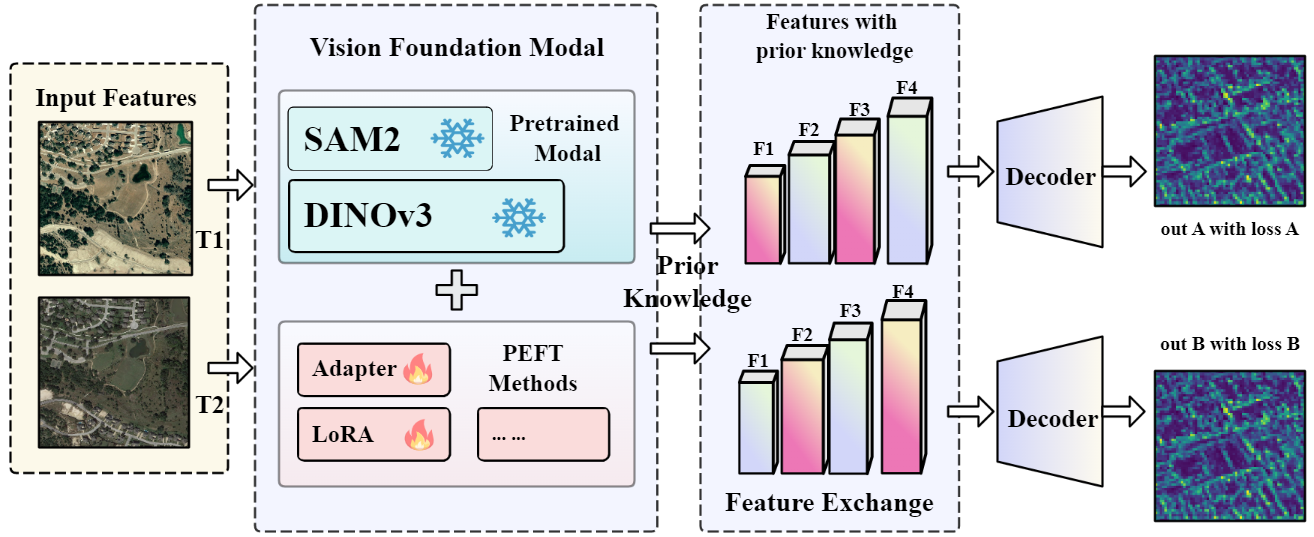
\includegraphics[width=\textwidth]{paper_figures/基于AI基础模型微调的变化检测模型研究/PeftCD/peftcd_framework.png}
  \caption{PeftCD 架构示意图。双时相影像通过注入 PEFT 模块的共享视觉基础模型编码器进行特征提取,特征在解码前进行交换,最终生成变化检测图。}
  \label{fig:peftcd_framework}
\end{figure}

基于上述动机,本节提出了一种基于 VFM 微调的全新变化检测框架——\textbf{PeftCD(Parameter-Efficient Fine-Tuning Change Detection)}。如图~\ref{fig:peftcd_framework}所示,我们选取了两类具有代表性的 VFMs 作为骨干:具备强大分割先验的 \textbf{Segment Anything Model v2 (SAM2)},以及自监督表征学习模型 \textbf{DINOv3}。在此基础上,我们引入了两种典型的 PEFT 方法:\textbf{LoRA}~\cite{LORA} 与 \textbf{Adapter}~\cite{adapter},以实现对遥感场景的高效适配。值得注意的是,除适配外,我们进一步观察到,ViT 类骨干(如 DINOv3)在经过 patch embedding 之后会以固定分辨率进行特征表示,缺乏类似 FPN 的多尺度金字塔结构,这在直接应用于像素级 RSCD 时容易导致边界模糊与伪变化敏感性。为释放其潜力,我们设计了 \textbf{多层融合与上下文增强(Multi-layer Fusion and Context Enhancement, MFCE)解码器},其结构如图~\ref{fig:peftcd_dino3cd} 所示。MFCE 在同尺度下实现跨 Transformer 层的深度注意力融合,并通过 ASPP 风格的上下文模块增强感受野。MFCE 解码器在不引入复杂解码头的前提下,有效补充了 DINOv3 的语义表征能力。而在另一实例中,SAM2 的实现(SAM2CD;见图~\ref{fig:peftcd_sam2cd})则结合了 FPN 与轻量级 ResBlock 解码器,更好地利用其分割先验。

\subsection{视觉基础模型简介}

\subsubsection{分割基础模型:SAM2}
Segment Anything Model 2 (SAM2)~\cite{ravi2024sam} 是原始 SAM~\cite{Kirillov2023SegmentA} 的一次重大升级,旨在提供更高质量且更高效的交互式与自动化图像分割。SAM2 在包含超过 11 亿分割掩膜的 SA-1B 数据集上进行训练,从而学习到丰富的目标结构、边界以及层次关系。与传统的分割模型不同,SAM2 的核心在于其可提示分割(promptable segmentation)能力,即模型能够根据点、边界框、掩膜或文本等多种提示,对图像中的任意目标进行分割。即使在缺少提示的情况下,模型也能自动生成场景中所有目标的分割结果。

在变化检测任务中,分割的本质是对目标边界进行精确刻画,以识别新增、消失或形态发生变化的对象。得益于大规模训练,SAM2 在边界捕获方面展现出卓越的能力,这与变化检测的核心需求高度契合。尤其是在建筑物、道路或水体的细粒度变化场景中,SAM2 可作为强有力的先验知识来源,提供高质量的目标级空间线索,从而提升整体的分割精度。

\subsubsection{自监督表征学习模型:DINOv3}
DINOv3~\cite{simeoni2025dinov3} 代表了自监督视觉 Transformer 的最新进展,标志着大规模无标签数据学习的前沿。不同于依赖人工标注的监督学习,自监督学习直接从数据本身中提取监督信号(如预测图像的被遮挡 patch),迫使模型在无标签条件下学习更加本质且鲁棒的表征。DINOv3 借鉴了 iBOT~\cite{Zhou2021iBOTIB} 等先进范式,并在高达 170 亿张无标签图像上进行训练,从而获得了可广泛迁移至多样化视觉任务的通用语义特征。

这些特征不仅具备强大的语义判别能力,同时对光照、视角或颜色变化的敏感性较低,更稳定地反映了目标的结构与语义属性。在遥感影像变化检测任务中,这种鲁棒性尤为关键。季节变换、光照差异与气候波动往往会引入大量伪变化,而传统基于特征的模型容易将其误判为真实变化。相比之下,DINOv3 通过自监督学习得到的表征能够有效抑制由外观变化引起的干扰,从而更准确地区分真实的地物覆盖变化与环境噪声,为变化检测提供稳定可靠的特征支持。


\subsection{参数高效微调方法}

为了有效地将基础模型适配于遥感变化检测任务,本节引入了两种具有代表性的参数高效微调(Parameter-Efficient Fine-Tuning, PEFT)方法:低秩适配(LoRA)~\cite{LORA} 和 Adapter~\cite{adapter}。

\subsubsection{低秩适配(LoRA)}

LoRA~\cite{LORA} 假设下游任务适配所需的权重更新可以通过低秩分解进行良好近似。设原始投影权重为 $\mat{W}_0\in\mathbb{R}^{d\times k}$。通过冻结 $\mat{W}_0$,引入一个低秩增量:
\begin{equation}
\Delta \mat{W}=\frac{\alpha}{r}\,\mat{B}\mat{A},\qquad
\mat{A}\in\mathbb{R}^{r\times k},\;\mat{B}\in\mathbb{R}^{d\times r},\;r\ll\min(d,k)
\end{equation}
从而得到更新后的权重:
\begin{equation}
\widehat{\mat{W}}=\mat{W}_0+\Delta \mat{W}
\end{equation}
前向传播可表示为:
\begin{equation}
\vect{h}=\widehat{\mat{W}}\,\vect{x}
=\mat{W}_0\vect{x}+\frac{\alpha}{r}\,\mat{B}\mat{A}\,\vect{x}
\end{equation}
在训练过程中,仅有 $\mat{A}$ 和 $\mat{B}$(以及可选的缩放超参数 $\alpha$)会被更新,而 $\mat{W}_0$ 保持冻结不变。在本节中,LoRA 模块被注入到 Transformer 的多头自注意力(Multi-Head Self-Attention, MHSA)中的特定线性投影部分。其超参数设置为 $r{=}8$,$\alpha{=}32$。LoRA 的优势在于其简洁高效,仅引入少量额外参数,却能够有效引导模型朝向任务相关的表征。

\subsubsection{Adapter}

Adapter~\cite{adapter} 是最早提出的 PEFT 方法之一。其核心思想是在每个 Transformer 块内部,以与主干网络并行的方式插入一个轻量级的“瓶颈”结构。典型的 Adapter 模块由一个降维全连接层、一个非线性激活函数(如 GELU),以及一个升维全连接层构成。在前向传播中,输入特征首先通过降维投影进行压缩,再经过非线性激活,最后通过升维投影恢复维度,并通过残差连接与原始特征相加。Adapter 的灵活性在于其插入位置的多样性,可以在特定层增强任务适应性,因此特别适合定制化微调。其计算过程可表示为:
\begin{equation}
    h_{\text{Adapter}}(x) = W_{\text{up}} f(W_{\text{down}} x) + x,
    \label{eq:adapter}
\end{equation}
其中 $x$ 表示 Transformer 块的输出,$f$ 为非线性激活函数。在微调过程中,仅有 Adapter 模块的内部权重 $W_{\text{down}}$ 与 $W_{\text{up}}$ 会被更新。Adapter 的优势在于其结构灵活且模块化,能够方便地集成至任意层的现有模型中。


\begin{table}[!htbp]
\centering
\caption{PeftCD 所用的 PEFT 配置。LoRA 设置 \textbf{dropout}=0.1,注入于 \texttt{qkv} 投影层。所有编码器权重均被冻结,仅 PEFT 模块可训练。Adapter 在每个编码器块前插入残差 MLP 结构。}
\label{tab:peftcd_cfg}
\begin{tabular}{l l l c c}
\toprule
\textbf{Backbone} & \textbf{Strategy} & \textbf{Injected Layers} & \textbf{Rank/Dim} & \textbf{Scale $\alpha$} \\
\midrule
SAM2   & LoRA    & MHSA (\texttt{qkv})    & r=8   & 32 \\
SAM2   & Adapter & Pre-block    & dim=32 & -- \\
DINOv3 & LoRA    & MHSA (\texttt{qkv})     & r=8   & 32 \\
DINOv3 & Adapter & Pre-block     & dim=32 & -- \\
\bottomrule
\end{tabular}
\end{table}

\begin{figure}[!htbp]
  \centering
  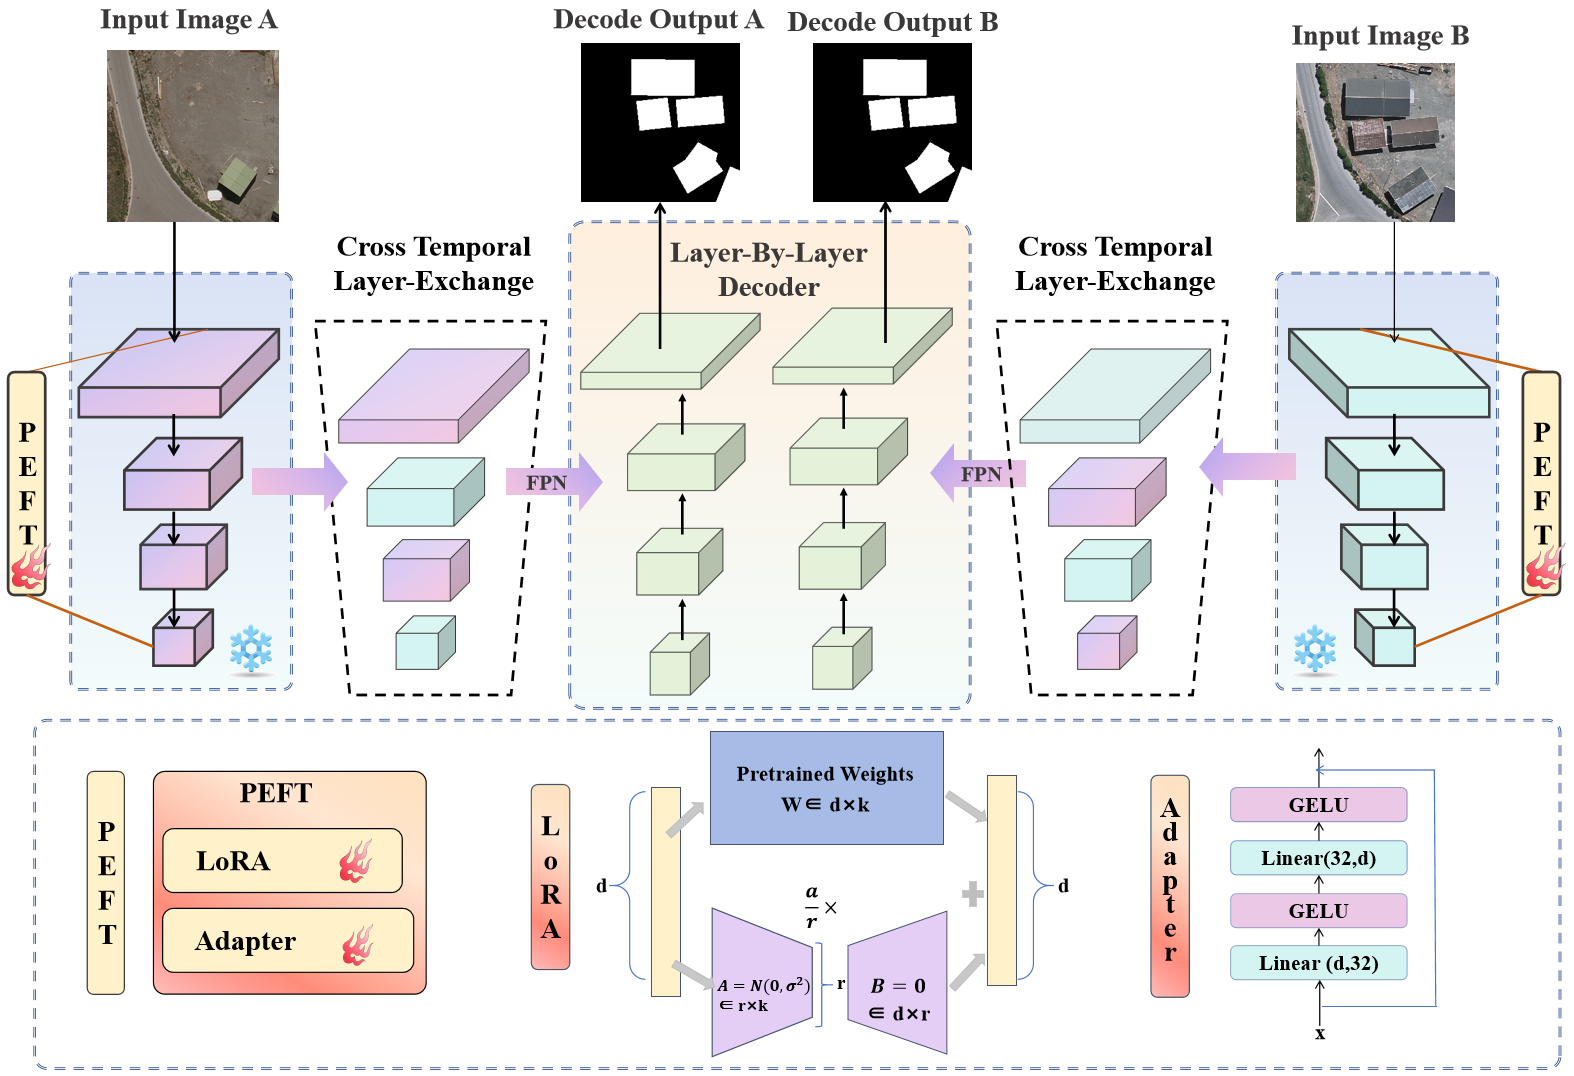
\includegraphics[width=\textwidth]{paper_figures/基于AI基础模型微调的变化检测模型研究/PeftCD/peftcd_sam2cd.png}
  \caption{基于 SAM2 的 PeftCD 模型架构示意图(SAM2CD)。双时相影像输入共享的、插入了PEFT模块的SAM2编码器。提取的特征金字塔经过特征交换后,送入共享的解码器,最终生成变化图。}
  \label{fig:peftcd_sam2cd}
\end{figure}


\subsection{PeftCD模型架构}

\subsubsection{整体思路}

所提出的 PeftCD 框架如图~\ref{fig:peftcd_framework} 所示,基础的变化检测范式采用前文提及的SEED架构。对于一对双时相遥感影像 $X_t$ 和 $X_{t'}$,首先通过共享权重的骨干网络(可选 SAM2 或 DINOv3)提取特征表示。在实验中,我们采用 \texttt{sam2\_hiera\_large} 与 \texttt{dinov3\_vitl16} 作为骨干网络。  
\textbf{参数高效适配}的具体配置如表~\ref{tab:peftcd_cfg} 所示:(i) LoRA被注入至每一个Transformer 块的多头自注意力(MHSA)\texttt{qkv} 投影中,设置秩 $r{=}8$、缩放系数 $\alpha{=}32$、dropout 为 $0.1$;(ii) Adapter则对 每一个编码器块进行封装,采用前置残差 MLP 结构(两层瓶颈结构,激活函数为 GELU,瓶颈维度为 $32$)。在两种策略下,所有骨干网络的参数保持冻结,仅有 PEFT 模块可训练。在编码之后,我们在双时相特征流之间引入特征层交换操作,以促进模型学习与变化相关的表征。交换后的特征再通过一个刻意设计的轻量化解码头进行解码,从而凸显 VFM 骨干网络的表征能力。在基于 SAM2 的架构中,我们采用 FPN 融合特征金字塔,并结合基于 ResBlock 的渐进式上采样解码器生成预测图。而在基于 DINOv3 的架构中,由于其输出为单尺度的高维语义特征,我们设计了解码器,先进行同尺度的多层特征融合与上下文增强(ASPP),再逐步上采样至原始分辨率。

\subsubsection{双时相特征处理与变化检测范式}
在特征交互和解码阶段,PeftCD框架采纳了本文在第六章中提出的SEED(Siamese-Encoder-Exchange-Decoder)范式。我们认为,这种摒弃了显式差异计算的架构,能够最大程度地保留基础模型提取的原始特征信息,充分发挥其强大的表征能力。
\begin{itemize}
    \item \textbf{孪生编码器 (Siamese Encoder):} 双时相影像 $X_t$ 和 $X_{t'}$ 分别通过同一个PEFT微调后的VFM编码器,生成两组多尺度特征金字塔 $\{F_t^i\}_{i=1}^L$ 和 $\{F_{t'}^i\}_{i=1}^L$。权重共享确保了对两幅影像的特征提取具有一致性。
    \item \textbf{特征交换 (Feature Exchange):} 在进入解码器之前,两组特征金字塔进行特征层交换(Layer-Exchange)。例如,奇数层的特征保持不变,偶数层的特征进行交换,从而生成两组混合了双时相信息的特征金字塔。
    \item \textbf{孪生解码器 (Siamese Decoder):} 两组混合特征金字塔分别输入到共享权重的孪生解码器中。解码器通过跳跃连接融合来自编码器的浅层空间信息,并逐层上采样恢复分辨率。最终,两个解码器分支都输出一个变化概率图。在训练时,两个输出都受到同一真实变化标签的监督。
\end{itemize}
在该范式下,模型被训练来识别由特征交换所引入的“时空特征不一致性”,这种不一致性在变化区域表现得尤为剧烈,从而使模型能够隐式地学习到变化的概念。

\begin{figure}[!htb]
  \centering
  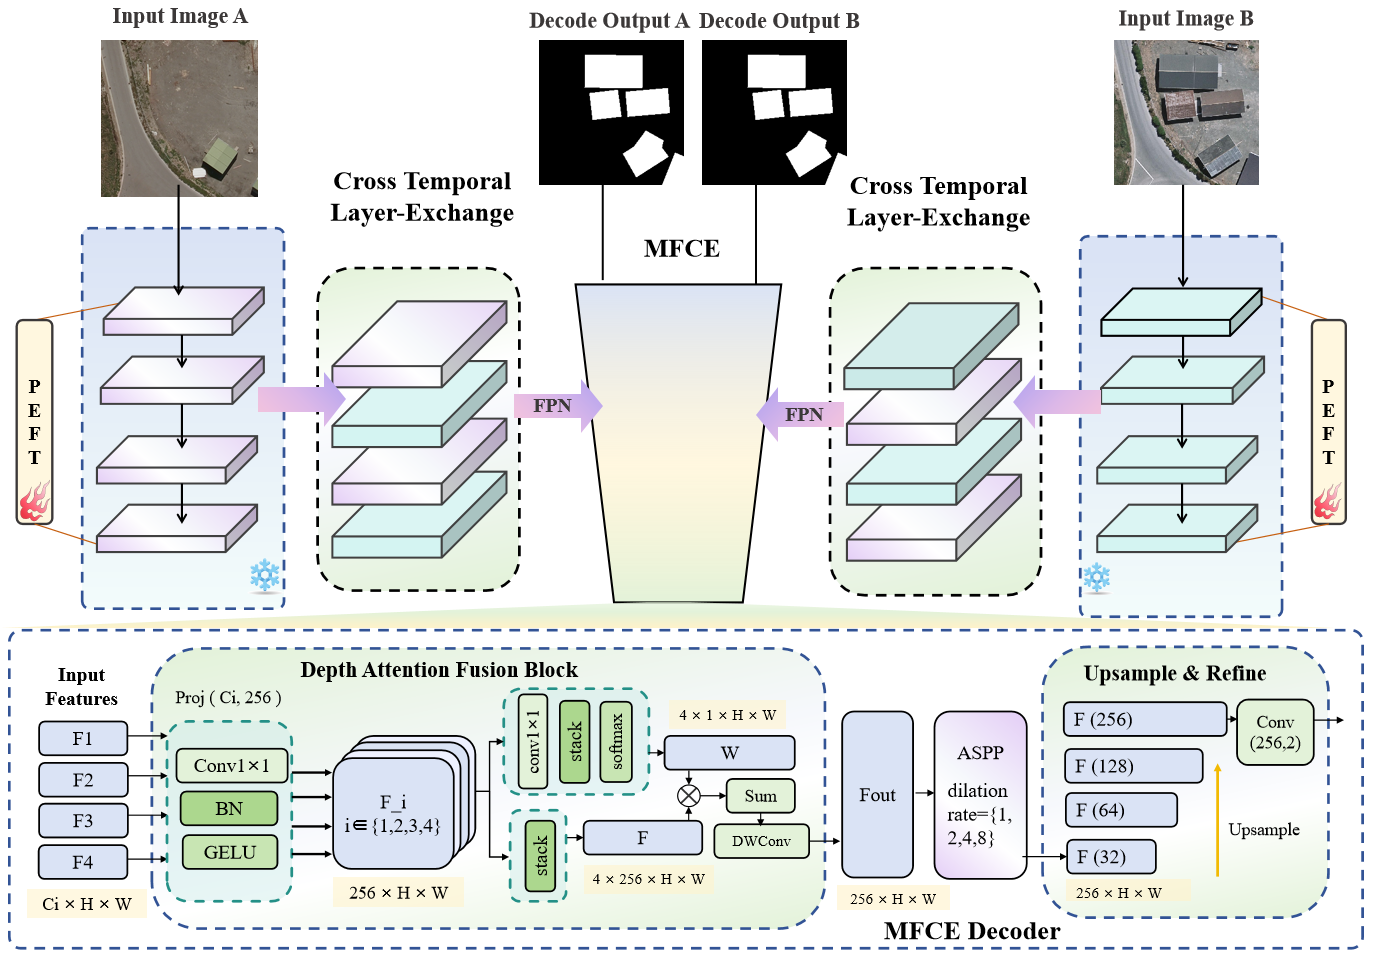
\includegraphics[width=\textwidth]{paper_figures/基于AI基础模型微调的变化检测模型研究/PeftCD/peftcd_dino3cd.png} % 请确保图片路径正确
  \caption{基于DINOv3的PeftCD模型架构(DINO3CD)。该模型采用与SAM2CD类似的SEED范式,但其核心编码器替换为DINOv3,旨在利用其强大的自监督表征来提升对伪变化的鲁棒性。}
  \label{fig:peftcd_dino3cd}
\end{figure}

\subsubsection{基于 SAM2 的 PeftCD架构}

为了将SAM2强大的分割先验知识有效迁移至遥感变化检测任务,我们设计了如图~\ref{fig:peftcd_sam2cd}所示的SAM2CD模型架构。该架构是PeftCD框架的一个具体实现,其核心在于将参数高效微调(PEFT)技术与本文提出的SEED变化检测范式深度融合。

\paragraph{孪生编码器与PEFT注入}
该模型采用孪生编码器(Siamese Encoder)结构来处理双时相输入 $T_1$ 与 $T_2$。其编码器骨干为共享权重的 SAM2 图像编码器,构建于 Vision Transformer (ViT) 之上,能够捕获图像的全局上下文信息。为了在不改变其大规模预训练参数的前提下,将 SAM2 适配于变化检测任务,我们在每个 Transformer 块中注入 PEFT 模块(LoRA 或 Adapter)。具体而言,在每个 Transformer 块中,我们将 LoRA 添加到 MHSA 的 \texttt{qkv} 投影中,参数设置为 $(r{=}8,\ \alpha{=}32,\ \text{dropout}{=}0.1)$;或者,替代性地,用一个前置残差 Adapter MLP(瓶颈维度为 $32$,激活函数为 GELU)对该块进行封装。所有原始的 SAM2 参数保持冻结,仅更新 LoRA/Adapter 的参数。这样的设计既保留了 SAM2 的强边界感知先验,又能高效地引导表征朝向双时相变化特征。  

编码器在每个时相生成一组多尺度特征金字塔。该设计既能保留 SAM2 的通用分割能力,又能高效学习针对双时相遥感影像的判别性特征,从而为后续的变化识别奠定基础。最终,编码器输出两组多尺度特征金字塔,分别以层次化的方式表征对应时相图像,从低层纹理到高层语义。  


\begin{table}[!htb]
\centering
\caption{PeftCD 与经典变化检测模型在 SYSU-CD 数据集上的定量对比结果}
\label{tab:peftcd_sysu}
\begin{tabular}{l c c c c c}
\toprule
\textbf{Model} & \textbf{OA} & \textbf{IoU} & \textbf{F1} & \textbf{Rec} & \textbf{Prec} \\
\midrule
STANet~\cite{chen_spatial-temporal_2020} & 88.24 & 57.22 & 72.79 & 66.71 & 80.08 \\
DSAMNet~\cite{shi_deeply_2022} & -- & 64.18 & 78.18 & 81.86 & 74.81 \\
BIT~\cite{chen_remote_2022} & 90.64 & 66.03 & 79.54 & 77.13 & 82.10 \\
P2V~\cite{lin_transition_2023} & 90.49 & 66.29 & 79.73 & 79.29 & 80.17 \\
HATNet~\cite{Xu2024HybridAT} & 90.92 & 67.00 & 80.24 & 78.23 & 82.36 \\
DARNet~\cite{li_densely_2022} & 91.26 & 68.10 & 81.03 & 79.11 & 83.04 \\
SSANet~\cite{Jiang2022JointVL} & -- & 68.18 & 81.08 & 79.73 & 82.48 \\
CDNeXt~\cite{wei_robust_2024} & 91.99 & 68.57 & 81.36 & 74.10 & 90.20 \\
BASNet~\cite{z_wang_bitemporal_2024} & 91.80 & 69.71 & 82.15 & 80.01 & 84.41 \\
ChangeCLIP~\cite{dong2024changeclip} & 92.08 & 70.53 & 82.72 & 80.41 & 85.16 \\
AGFormer~\cite{Chen2025AGFormerAA} & 92.04 & 70.91 & 82.98 & 82.26 & 83.71 \\
SGSLN~\cite{zhao_exchanging_2023} & -- & 71.05 & 83.07 & 81.45 & 84.76 \\
ChangeMamba~\cite{chen2024changemamba} & 92.30 & 71.10 & 83.11 & 80.31 & 86.11 \\
DEDANet~\cite{Li2025DifferenceEA} & 92.01 & 71.12 & 83.12 & 83.45 & 82.79 \\
DMFANet~\cite{Zhan2025DifferenceAwareMF} & 92.33 & 71.27 & 83.23 & 80.72 & 85.90 \\
UA-BCD~\cite{li_overcoming_2025} & -- & 71.38 & 83.30 & 79.66 & 87.28 \\
DgFA~\cite{f_zhou_dual-granularity_2025}   & 92.42 & 71.86 & 83.63 & 82.08 & 85.24 \\
FTA-Net~\cite{t_zhu_fta-net_2025}   & -- & 72.54 & 84.08 & 82.33 & 85.91 \\
CWmamba~\cite{Liu2025CWmambaLC} & 92.96 & 72.90 & 84.33 & 80.27 & 88.82 \\
SAM-Mamba~\cite{Li2025SAMMambaATC}  & -- & 73.09 & 84.45 & 83.79 & 85.12 \\
DepthCD~\cite{Zhou2025DepthCDDP}   & -- & 73.33 & 84.61 & 83.83 & 85.41 \\
CD-STMamba~\cite{Liu2025CDSTMambaTR} & 93.01 & 73.45 & 84.70 & 82.04 & 87.53 \\
\midrule
PeftCD(DINOv3)  & 93.25 & 73.81 & 84.93 & 80.71 & 89.61 \\
\bottomrule
\end{tabular}
\end{table}

\begin{figure}[!htb]
  \centering
  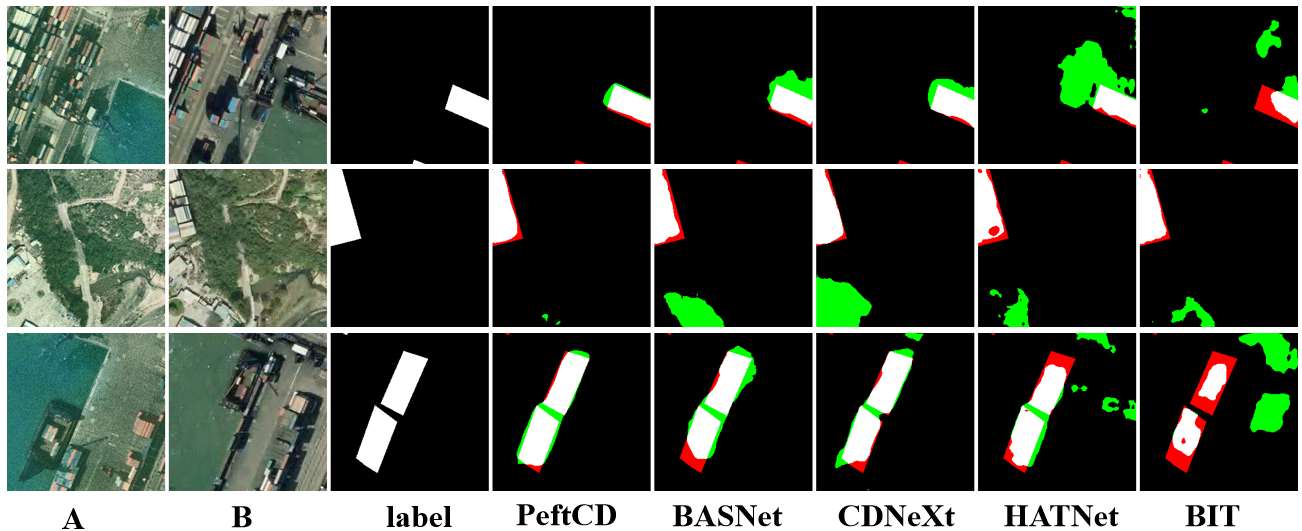
\includegraphics[width=\textwidth]{paper_figures/基于AI基础模型微调的变化检测模型研究/PeftCD/peftcd_sysu.png}
  \caption{PeftCD 模型与对比模型在 SYSU-CD 数据集上的可视化对比结果}
  \label{fig:peftcd_sysu}
\end{figure}


\begin{table}[!htb]
\centering
\caption{PeftCD 与经典变化检测模型在 WHUCD 数据集上的定量对比结果}
\label{tab:peftcd_whucd}
\begin{tabular}{l c c c c c}
\toprule
\textbf{Model} & \textbf{OA} & \textbf{IoU} & \textbf{F1} & \textbf{Rec} & \textbf{Prec} \\
\midrule
P2V~\cite{lin_transition_2023} & 99.31 & 85.91 & 92.42 & 90.93 & 93.97 \\
DSIFN~\cite{Zhang2020ADS} & 99.34 & 86.36 & 92.68 & 90.20 & 95.30 \\
MSCANet~\cite{m_liu_cnn-transformer_2022} & 99.36 & 86.65 & 92.85 & 89.98 & 95.90 \\
SGSLN~\cite{zhao_exchanging_2023} & 99.38 & 87.47 & 93.32 & 92.91 & 93.72 \\
BIT~\cite{chen_remote_2022} & 99.43 & 88.22 & 93.74 & 92.00 & 95.56 \\
HCGMNet~\cite{Han2023HCGMNetAH} & 99.52 & 90.10 & 94.79 & 95.31 & 94.27 \\
ChangeCLIP~\cite{dong2024changeclip} & 99.52 & 90.15 & 94.82 & 94.02 & 95.63 \\
CDNeXt~\cite{wei_robust_2024} & 99.54 & 90.35 & 94.93 & 92.56 & 97.43 \\
CGNet~\cite{han_change_2023} & 99.54 & 90.41 & 94.96 & 94.61 & 95.32 \\
EfficientCD~\cite{dong_efficientcd_2024} & 99.55 & 90.71 & 95.13 & 94.19 & 96.08 \\
SAFDNet~\cite{Fu2025BeyondCD} & 99.55 & 90.73 & 95.14 & 94.47 & 95.82 \\
\midrule
PeftCD & 99.62 & 92.05 & 95.86 & 94.95 & 96.79 \\
\bottomrule
\end{tabular}
\end{table}

\begin{figure}[!htb]
  \centering
  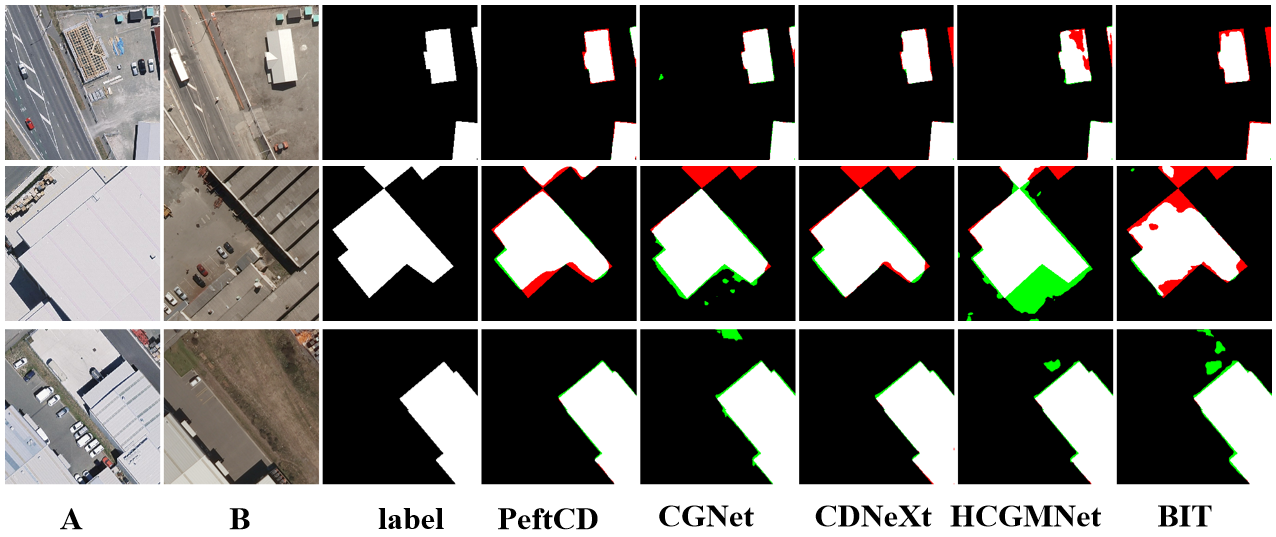
\includegraphics[width=\textwidth]{paper_figures/基于AI基础模型微调的变化检测模型研究/PeftCD/peftcd_whucd.png}
  \caption{PeftCD 模型与对比模型在 WHUCD 数据集上的可视化对比结果}
  \label{fig:peftcd_whucd}
\end{figure}



\begin{table}[!htb]
\centering
\caption{PeftCD 与经典变化检测模型在 S2Looking 数据集上的定量对比结果}
\label{tab:peftcd_s2looking}
\begin{tabular}{l c c c c c}
\toprule
\textbf{Model} & \textbf{OA} & \textbf{IoU} & \textbf{F1} & \textbf{Rec} & \textbf{Prec} \\
\midrule
HATNet~\cite{Xu2024HybridAT} & - & 47.08 & 64.02 & 60.90 & 67.48 \\
FHD~\cite{pei_feature_2022} & - & 47.33 & 64.25 & 56.71 & 74.09 \\
BIT~\cite{chen_remote_2022} & - & 47.94 & 64.81 & 58.15 & 73.20 \\
SAM-CD~\cite{ding2024adapting} & - & 48.29 & 65.13 & 58.92 & 72.80 \\
DMINet~\cite{feng_change_2023} & - & 48.33 & 65.16 & 62.13 & 68.51 \\
AEGL-Net~\cite{Ying2025AEGLNetAM} & - & 48.36 & 65.19 & 60.69 & 70.05 \\
HFIFNet~\cite{Han2025HFIFNetHF} & 99.22 & 48.54 & 65.35 & 61.04 & 70.33 \\
SGANet~\cite{j_chen_sganet_2025} & - & 48.72 & 66.01 & 57.26 & 77.91 \\
CDNeXt~\cite{wei_robust_2024} & - & 50.05 & 66.71 & 63.08 & 70.78 \\
AGFormer~\cite{Chen2025AGFormerAA} & 99.21 & 50.14 & 66.80 & 65.31 & 68.35 \\
Changer~\cite{Fang2022ChangerFI} & - & 50.47 & 67.08 & 62.04 & 73.01 \\
CWmamba ~\cite{Liu2025CWmambaLC} & 99.24 & 51.43 & 67.93 & 66.19 & 68.38 \\
Conv-former~\cite{Yang2025ConvFormerCDHC} & 99.21 & 51.51 & 68.00 & 62.81 & 74.12 \\
PeftCD & 99.30 & 52.25 & 68.64 & 63.53 & 74.64 \\
\bottomrule
\end{tabular}
\end{table}


\begin{figure}[!htb]
  \centering
  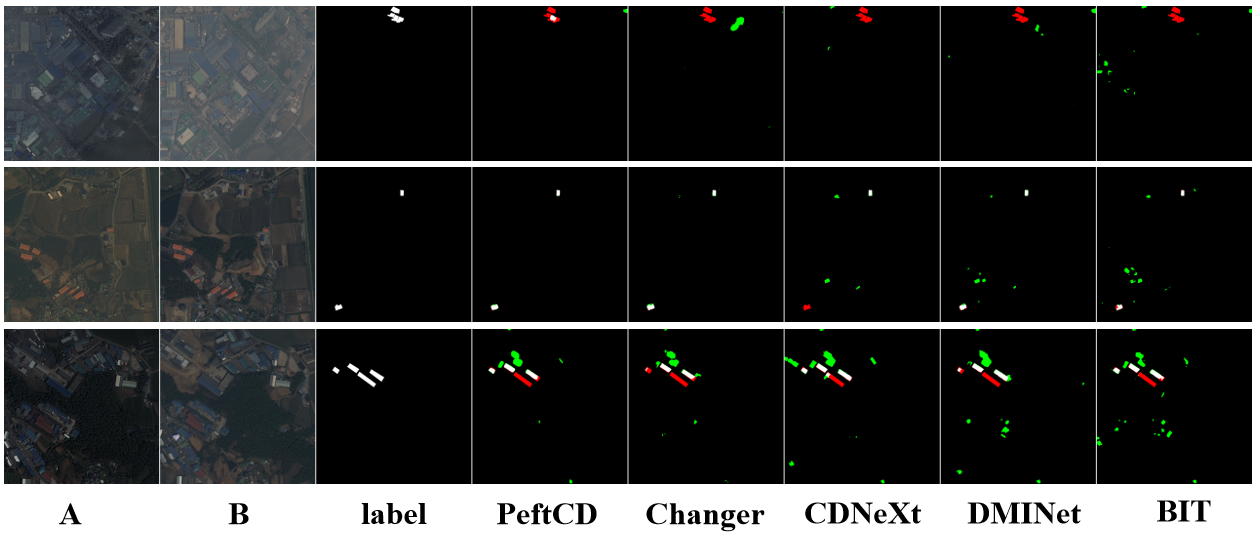
\includegraphics[width=\textwidth]{paper_figures/基于AI基础模型微调的变化检测模型研究/PeftCD/peftcd_s2looking.png}
  \caption{PeftCD 模型与对比模型在 S2Looking 数据集上的可视化对比结果}
  \label{fig:peftcd_s2looking}
\end{figure}



\paragraph{基于交换的特征交互}
在特征交互阶段,我们遵循SEED范式,摒弃了传统的差异计算模块(如特征相减或拼接融合),转而采用特征层交换(Feature Layer Exchange)机制。具体而言,从编码器输出的两组特征金字塔中,部分层级(例如,偶数层)的特征图在两个处理流之间进行交换,而其他层级(例如,奇数层)则保持不变。通过这种方式,我们得到了两组新的“混合时相”特征金字塔。这一操作的核心目的,是为后续的解码器创造一个必须解决“时空特征不一致性”的学习任务。随后,这两组混合特征金字塔被送入一个共享权重的特征金字塔网络(Shared FPN),以增强跨尺度的特征融合,为解码阶段提供更丰富的特征表示。

\paragraph{孪生解码与监督}
解码阶段同样采用共享权重的孪生解码器(Siamese Decoder)结构。每个解码器分支接收来自FPN的混合时相特征,并基于 ResBlock 构建特征提取,从而以逐层上采样的方式进行逐层特征优化和解码。
\begin{itemize}
    \item 对于未变化区域,两个时相的特征在语义和空间上高度一致,即使经过交换,解码器也能顺利重构,输出低变化概率。
    \item 对于变化区域,解码器会面临剧烈的特征冲突(例如,用“植被”的空间细节去重构“建筑”的语义),这种不一致性正是模型学习识别为“变化”的强大监督信号。
\end{itemize}
最终,两个解码器分支分别输出一个变化概率图。在训练时,这两个输出图同时受到同一个真实变化标签(Change Mask)的监督。在推理阶段,则将两个输出图进行逐像素平均,以获得更稳定和鲁棒的最终变化检测结果。



\begin{table}[!htbp]
\centering
\caption{PeftCD 与经典变化检测模型在 MSRSCD 数据集上的定量对比结果}
\label{tab:peftcd_msrscd}
\begin{tabular}{l c c c c c}
\toprule
\textbf{Model} & \textbf{OA} & \textbf{IoU} & \textbf{F1} & \textbf{Rec} & \textbf{Prec} \\
\midrule
STANet~\cite{chen_spatial-temporal_2020} & 91.44 & 54.52 & 70.57 & 69.46 & 71.71 \\
SGSLN~\cite{zhao_exchanging_2023} & 92.52 & 56.28 & 73.36 & 69.73 & 77.39 \\
ChangeFormer~\cite{bandara2022transformer} & 91.86 & 56.96 & 72.58 & 72.94 & 72.22 \\
FCCDN~\cite{Chen2021FCCDNFC} & 92.36 & 57.94 & 73.37 & 71.30 & 75.56 \\
AANet~\cite{Hang2024AANetAA} & 92.17 & 59.23 & 74.40 & 77.03 & 71.94 \\
EATDer~\cite{Ma2024EATDerEA} & 91.47 & 59.29 & 74.44 & 84.17 & 66.73 \\
MSNet~\cite{Liu2025NetworkAD} & 93.03 & 59.80 & 75.74 & 74.73 & 76.79 \\
DMINet~\cite{feng_change_2023} & 93.05 & 61.24 & 75.96 & 74.37 & 77.63 \\
BASNet~\cite{z_wang_bitemporal_2024} & 92.87 & 61.31 & 76.02 & 76.51 & 75.53 \\
CDNeXt~\cite{wei_robust_2024} & 93.24 & 61.59 & 76.23 & 73.42 & 79.27 \\
DFFNet~\cite{Liu2025FullScaleCD} & 93.23 & 61.82 & 77.44 & 78.69 & 76.22 \\
\midrule
PeftCD & 93.83 & 64.07 & 78.10 & 74.19 & 82.44 \\
\bottomrule
\end{tabular}
\end{table}


\begin{figure}[!htb]
  \centering
  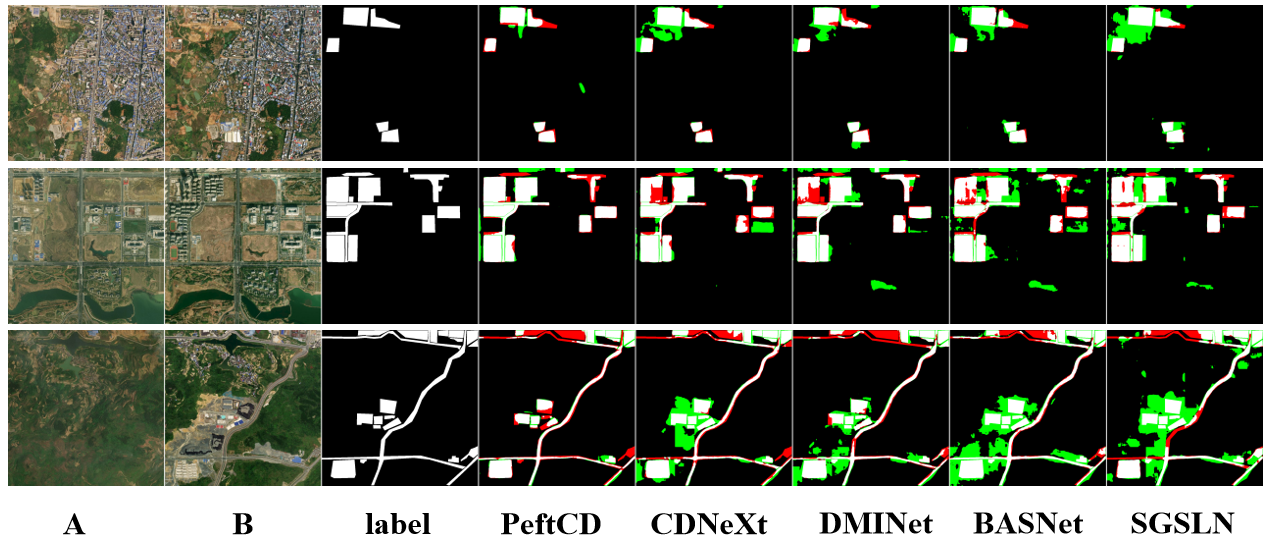
\includegraphics[width=\textwidth]{paper_figures/基于AI基础模型微调的变化检测模型研究/PeftCD/peftcd_msrscd.png}
  \caption{PeftCD 与对比模型在 MSRSCD 数据集上的可视化对比结果.}
  \label{fig:peftcd_msrscd}
\end{figure}


\begin{table}[!htb]
\centering
\caption{PeftCD 与经典变化检测模型在 MLCD 数据集上的定量对比结果}
\label{tab:peftcd_mlcd}
\begin{tabular}{l c c c c c}
\toprule
\textbf{Model} & \textbf{OA} & \textbf{IoU} & \textbf{F1} & \textbf{Rec} & \textbf{Prec} \\
STANet~\cite{chen_spatial-temporal_2020}         & 86.97 & 60.87 & 75.67 & 73.4  & 78.09 \\
ISDANet~\cite{h_ren_interactive_2025}            & 88.3  & 66.52 & 79.89 & 84.2  & 76    \\
EFI-SAM~\cite{Huang2025SAMBasedEF}          & -- & 67.72 & 80.75 & -- & -- \\
DARNet~\cite{li_densely_2022}         & 90.24 & 69.05 & 81.69 & 78.84 & 84.75 \\
BASNet~\cite{z_wang_bitemporal_2024}         & 90.51 & 70.55 & 82.73 & 82.29 & 83.17 \\
BIT~\cite{chen_remote_2022}            & 91.23 & 72.02 & 83.73 & 81.74 & 85.83 \\
DMINet~\cite{feng_change_2023}         & 91.94 & 74.03 & 85.08 & 83.18 & 87.07 \\
\midrule
PeftCD & 92.94 & 76.89 & 86.93 & 85.02 & 88.94 \\
\bottomrule
\end{tabular}
\end{table}

\begin{figure}[!htb]
  \centering
  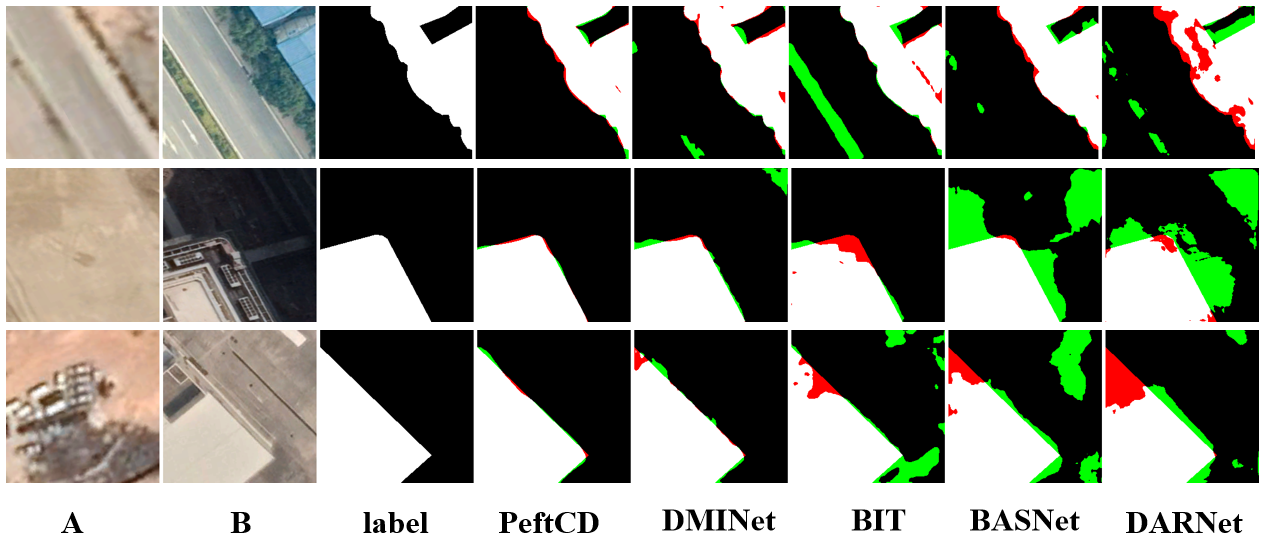
\includegraphics[width=\textwidth]{paper_figures/基于AI基础模型微调的变化检测模型研究/PeftCD/peftcd_mlcd.png}
  \caption{PeftCD 与对比模型在 MLCD 数据集上的可视化对比结果.}
  \label{fig:peftcd_mlcd}
\end{figure}


\subsubsection{基于 DINOv3 的 PeftCD架构}

我们还在 DINOv3 上实例化了 PeftCD(见图~\ref{fig:peftcd_dino3cd})。与 SAM2 不同,DINOv3 并非面向分割设计,其在 patch embedding 之后以固定空间分辨率进行运算,在各层中均输出同尺度特征。根据表~\ref{tab:peftcd_cfg} 的设置,每个 Transformer 块均通过 LoRA 注入至 MHSA 的 \texttt{qkv} 投影($r{=}8$, $\alpha{=}32$, dropout $0.1$),或通过前置残差 Adapter MLP(瓶颈维度 $32$,激活函数为 GELU)进行适配。在此过程中,骨干网络权重保持冻结,仅有 PEFT 模块参数参与训练。在使用共享权重对双时相图像进行编码后,我们执行特征层交换,以增强双时相之间的交互。解码器随后依次执行:(i) 同尺度多层特征的深度注意力融合;(ii) 基于 ASPP 的上下文增强;以及 (iii) 渐进式上采样,最终生成变化检测结果图。该设计弥补了 ViT 类骨干缺乏空间金字塔结构的不足,同时保留了 DINOv3 在语义表征和跨域泛化方面的优势。  



\subsection{基于同尺度多层融合与上下文增强的解码器}

传统的基于卷积神经网络(CNN)的编码器-解码器架构,通常依赖于编码器生成的多尺度特征金字塔(Feature Pyramid Network, FPN)。这些由不同下采样阶段产生的特征图,既包含了高层语义信息(深层、低分辨率特征),也保留了精细的空间细节(浅层、高分辨率特征),为解码器逐层恢复分辨率和精确分割提供了关键信息~\cite{lin_feature_2017}。

然而,当采用以 DINO 或其他视觉 Transformer(ViT)为代表的视觉基础模型作为编码器主干时,这一经典范式面临挑战。ViT 架构在初始的“块嵌入”(Patch Embedding)阶段,便将输入图像直接下采样 16 倍,并将图像块序列化。后续的所有 Transformer 块均在这一固定分辨率(例如 $H/16 \times W/16$)上进行特征变换与信息交互。虽然不同 Transformer 层的输出特征捕获了从低级到高级的不同层次语义,但它们在空间分辨率上是单一的,并未形成传统意义上的特征金字塔。这种架构特性导致解码器在进行上采样时,严重缺乏多尺度的空间信息,特别是对于恢复物体边界和细微变化至关重要的高频细节,从而可能导致预测结果边缘模糊、小目标丢失等问题。

为了解决 ViT 骨干网络缺乏特征金字塔的问题,我们设计了一种专门的解码器(Multi-Layer Fusion and Contextual Enhancement, MFCE)。该解码器不依赖于多尺度的空间输入,而是通过两个核心步骤,在单尺度特征图上构建强大的特征表示,并以此为基础进行上采样恢复。首先,为了在解码阶段充分利用不同层级的特征信息,对来自 ViT 不同层的同尺度特征进行深度注意力融合。其次,为了在解码阶段,扩展模型对影像特征的上下文理解能力,利用空洞空间金字塔池化(ASPP)模块构建感受野金字塔以增强上下文信息。由此,解码端的输入特征既融合了不同层级的特征信息,同时也获取了丰富的多尺度上下文感知能力。最后,解码器通过渐进式上采样路径,逐步恢复分辨率并生成最终的变化检测结果。

\subsubsection{同尺度多层特征的深度注意力融合}
尽管 ViT 的各层输出特征图分辨率相同,但它们在语义层面构成了“深度金字塔”。浅层特征更关注局部纹理和边缘,而深层特征则编码了更抽象的全局语义。为了充分且智能地利用这些信息,解码器的首要任务是对其进行高效融合。

我们为此设计了一个深度注意力融合模块,用以处理来自编码器不同层级的多个同尺度特征图。在本节中,参考ResNet与Swin Transformer等模型的架构设计方法,选用5,11,17,23层的输出作为同尺度特征图融合输入。对于输入的 4 个特征图 $\{F_1, F_2, F_3, F_4\}$,其中 $F_i \in \mathbb{R}^{B \times C_i \times H \times W}$,该模块首先将它们投影到统一的中间维度 $C_{mid}$,得到 $\{X_1, X_2, X_3, X_4\}$。随后,为每个空间位置 $(h, w)$ 的每个特征层 $X_i$ 学习一个注意力权重 $A_i(h, w)$。该权重由一个 $1 \times 1$ 卷积网络生成,并通过沿深度(层)维度的 Softmax 函数进行归一化:
\begin{equation}
    A_i(h, w) = \frac{\exp(S_i(h, w))}{\sum_{j=1}^{N} \exp(S_j(h, w))}
\end{equation}
其中 $S_i$ 是从 $X_i$ 生成的分数图。最终的融合特征 $\mathbf{X}_{\text{fused}}$ 是所有特征层的加权和:
\begin{equation}
    \mathbf{X}_{\text{fused}} = \sum_{i=1}^{N} A_i \odot X_i
\end{equation}
其中 $\odot$ 表示逐元素乘法。这种空间可变的深度注意力机制,使得模型能够根据每个像素的具体内容,自适应地决定更依赖于哪一层级的语义信息(是纹理还是类别),从而生成一个信息高度浓缩的、强大的单尺度特征图。

\subsubsection{上下文增强与渐进式上采样}
在特征融合之后,我们利用空洞空间金字塔池化(Atrous Spatial Pyramid Pooling, ASPP)模块进一步增强特征的上下文感知能力。ASPP 在融合后的特征图上并行应用多个不同膨胀率的深度可分离空洞卷积。这能够在不改变特征图分辨率的前提下,捕获多尺度的上下文信息,构建出一个“感受野金字塔”(receptive field pyramid),有效弥补了原始骨干网络在空间尺度多样性上的不足,为后续的上采样提供了更鲁棒的语义信息。

最后,经过上下文增强的特征图(分辨率仍为 $1/16$)将进入一个渐进式上采样路径。该路径通过三次“双线性插值上采样 + 深度可分离卷积”的组合,将分辨率从 $1/16$ 逐步提升至 $1/8$、$1/4$,并最终恢复到原始尺寸。其中的深度可分离卷积模块用于在上采样后平滑和优化特征,以此获取更丰富的细节信息。最终,由预测头生成像素级的变化检测结果。

\begin{table}[!htb]
\centering
\caption{PeftCD 与经典变化检测模型在 CDD 数据集上的定量对比结果}
\label{tab:peftcd_cdd}
\begin{tabular}{l c c c c c}
\toprule
\textbf{Model} & \textbf{OA} & \textbf{IoU} & \textbf{F1} & \textbf{Rec} & \textbf{Prec} \\
\midrule
BASNet~\cite{z_wang_bitemporal_2024} & 99.18 & 93.29 & 96.53 & 96.30 & 96.76 \\  
UA-BCD~\cite{li_overcoming_2025}     & --    & 93.49 & 96.64 & 96.90 & 96.38 \\
RCDT~\cite{lu_cross_2024}                  & --    & 93.79 & 96.80 & 96.97 & 96.63 \\
CDMamba~\cite{zhang_cdmamba_2025}    & 99.26 & 93.93 & 96.87 & 96.84 & 96.90 \\
SFFCE-CD~\cite{y_xing_sffce-cd_2025}   & 99.29 & 94.42 & 97.13 & 96.94 &  97.32 \\
ELGCNet~\cite{m_noman_elgc-net_2024}   & 99.33  &  94.50   & 91.17  & --   & -- \\   
DgFA~\cite{f_zhou_dual-granularity_2025} & 99.41 & 95.12 & 97.50 & 97.60 & 97.40 \\
GASNet~\cite{zhang_global-aware_2023}  & 99.41  & 95.34  & 97.61  & 98.06  & 97.17 \\
DEDANet~\cite{Li2025DifferenceEA} & 99.40 & 95.46 & 97.67 & 97.14 & 98.22 \\
DSCRNet ~\cite{Zhang2025ADS} & -- & 95.46 & 97.68 & 97.85 & 97.51 \\
CD-STMamba~\cite{Liu2025CDSTMambaTR} & 99.41 & 95.56 & 97.73 & 97.45 & 98.01 \\
MLDFNet~\cite{d_sidekejiang_mldfnet_2025}  & -- & 95.78 & 97.84 & 97.97 & 97.72 \\
ScratchFormer~\cite{Noman2023RemoteSC}   & 99.50 & 95.85  & 97.88 & -- & -- \\ 
FTransDF-Net~\cite{li_dual_2025}   & -- & 95.85 &  97.88 & 97.63 & 98.13 \\
DSFI-CD~\cite{x_li_dsfi-cd_2025}  & 99.52 & 96.10 &  98.01 & 98.34 & 97.68 \\
HASNet~\cite{c_tao_hasnet_2025}        & 99.56 & 96.49 & 98.21 & 98.12 & 98.32 \\
\midrule
PeftCD & 99.63 & 97.01 & 98.48 & 98.30 & 98.67 \\
\bottomrule
\end{tabular}
\end{table}

\begin{figure}[!htb]
  \centering
  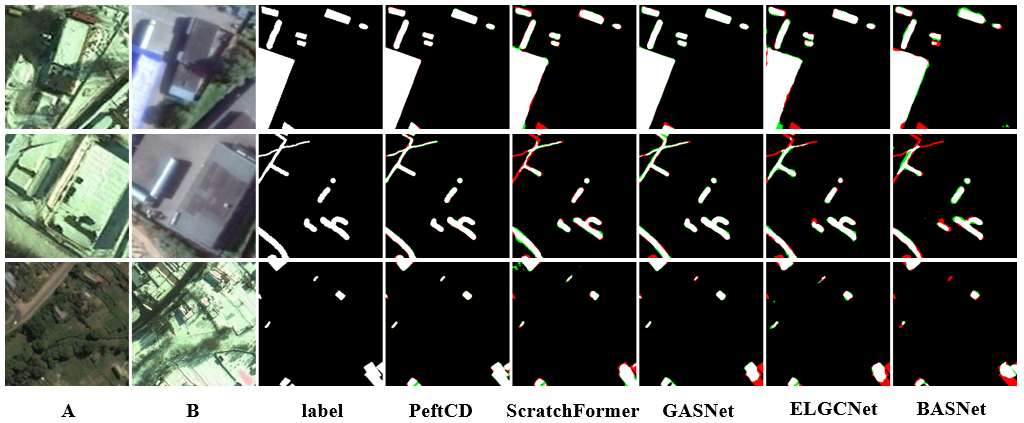
\includegraphics[width=\textwidth]{paper_figures/基于AI基础模型微调的变化检测模型研究/PeftCD/peftcd_cdd.png}
  \caption{PeftCD 与对比模型在 CDD 数据集上的可视化对比结果.}
  \label{fig:peftcd_cdd}
\end{figure}

\subsection{实验结果与分析}
\subsubsection{实验结果量化指标与可视化分析}

我们在七个具有挑战性的数据集上进行了全面的定量实验,包括 SYSU-CD、WHUCD、MSRSCD、CDD、S2Looking、LEVIR-CD 和 MLCD,以全面评估所提出 PeftCD 框架的有效性,并将其与具有代表性的先进变化检测方法进行对比。如表~\ref{tab:peftcd_sysu}、~\ref{tab:peftcd_whucd}、~\ref{tab:peftcd_s2looking}、~\ref{tab:peftcd_msrscd}、~\ref{tab:peftcd_mlcd}、~\ref{tab:peftcd_cdd} 和~\ref{tab:peftcd_levir} 所总结的结果显示,我们的方法具有显著的优越性。在所有数据集上,结合 PEFT 策略的 PeftCD 明显优于传统的 CNN 与 Transformer 基线模型,并在性能上达到或超过当前最先进方法(SOTA)。  

更具体而言,在 SYSU-CD、WHUCD、MSRSCD、CDD、S2Looking 和 MLCD 上,PeftCD 分别取得了 73.81\%、92.05\%、64.07\%、97.01\%、52.25\% 和 76.89\% 的 IoU,均超过了所有对比方法。在 SYSU-CD 上,PeftCD 将 IoU 提升 2.71 个百分点至 73.81\%,并实现了 84.93\% 的 F1 分数,显著高于亚军 ChangeMamba(83.11\%)。在 WHUCD 上,PeftCD 达到 92.05\% 的 IoU,超过 EfficientCD 1.34 个百分点,并获得 96.79\% 的 Precision,表明其对误报具有很强的抑制能力。在 S2Looking 上,PeftCD 取得了 52.25\% 的 IoU,优于 Conv-former(51.51\%)。这些结果表明,PeftCD 在复杂变化场景中表现出色,能够有效捕获多样化的变化模式。  



\begin{table}[!htb]
\centering
\caption{PeftCD 模型与经典变化检测模型在 LEVIR-CD 数据集上的定量对比结果}
\label{tab:peftcd_levir}
\begin{tabular}{l c c c c c}
\toprule
\textbf{Model} & \textbf{OA} & \textbf{IoU} & \textbf{F1} & \textbf{Rec} & \textbf{Prec} \\
\midrule
    STANet~\cite{chen_spatial-temporal_2020}   & 99.02 & 81.85 & 90.02 & 87.13 & 93.10 \\
    MSCANet~\cite{m_liu_cnn-transformer_2022}          &  99.03 &  81.91 &  90.06 &  86.38 &  94.06  \\
    MFATNet~\cite{Mao2022MFATNetMF}          &  99.03 &  82.42 &  90.36 &  88.93 &  91.85  \\
    ChangeFormer~\cite{bandara2022transformer}     &  99.04 &  82.66 &  90.50 &  90.18 &  90.83  \\
    P2V~\cite{lin_transition_2023}              &  99.04 &  83.00 &  90.71 &  91.78 &  89.67  \\
    CDMamba~\cite{zhang_cdmamba_2025}          &  99.06 &  83.07 &  90.75 &  90.08 &  91.43  \\
    AMTNet~\cite{Liu2023AnAM}           &   --   &  83.08 &  90.76 &  89.71 &  91.82  \\
    B2CNet~\cite{Zhang2024B2CNetAP} & 99.10 & 83.72 & 91.14 & 91.01 & 91.27 \\
    DgFA~\cite{f_zhou_dual-granularity_2025}   & 99.11 & 83.93 & 91.26 & 90.84 & 91.69 \\
    HATNet~\cite{Xu2024HybridAT} & 99.13 & 84.12 & 91.38 & 90.15 & 92.64 \\
    DMATNet~\cite{Song2022RemoteSI}          &  98.25 &  84.13 &  90.75 &  89.98 &  91.56  \\
    DEDANet~\cite{Li2025DifferenceEA}          &  99.14 &  84.18 &  91.41 &  90.06 &  92.80  \\
    STransUNet~\cite{Yuan2022STransUNetAS}       &  99.13 &  84.19 &  91.41 &  90.55 &  92.30  \\
    LCCDMamba~\cite{Huang2025LCCDMambaVS}       &  99.16 &  84.64 &  91.68 &  92.42 &  90.96  \\
    AGFormer~\cite{Chen2025AGFormerAA}         &  99.17 &  84.81 &  91.78 &  90.84 &  92.74  \\
    DSCRNet~\cite{Zhang2025ADS}         &  -- &  85.15 &  91.98 &  92.43 &  91.53  \\
    HCGMNet~\cite{Han2023HCGMNetAH}          &  99.18 &  85.26 &  92.04 &  92.81 &  91.29  \\
    Changer~\cite{Fang2022ChangerFI}        &   --   &  85.29 &  92.06 &  90.56 &  93.61  \\
    DMFANet~\cite{Zhan2025DifferenceAwareMF}         &  99.20 &  85.33 &  92.09 &  90.93 &  93.27  \\
    CGNet~\cite{han_change_2023}            &  99.20 &  85.40 &  92.13 &  91.93 &  92.32  \\
    EfficientCD~\cite{dong_efficientcd_2024} &  99.22 &  85.55 &  92.21 &  91.22 &  93.23  \\
    FTA-Net~\cite{t_zhu_fta-net_2025}   & -- & 85.58 & 92.23 & 92.68 & 91.79 \\
\midrule
PeftCD  & 99.22 & 85.62 & 92.25 & 91.44 & 93.08 \\
\bottomrule
\end{tabular}
\end{table}

\begin{figure}[!htb]
  \centering
  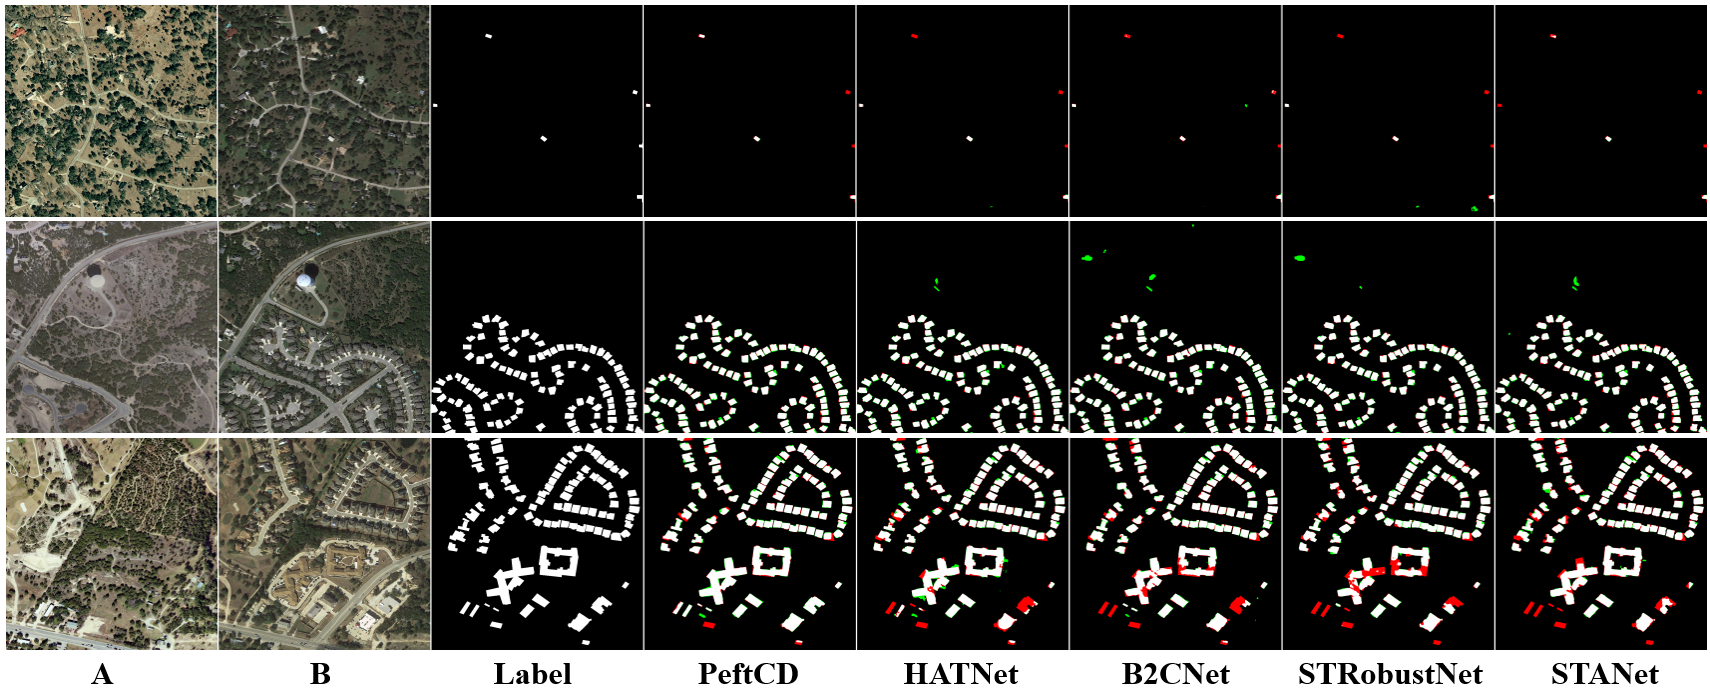
\includegraphics[width=\textwidth]{paper_figures/基于AI基础模型微调的变化检测模型研究/PeftCD/peftcd_levir.png}
  \caption{PeftCD 与对比模型在 LEVIR-CD 数据集上的可视化对比结果.}
  \label{fig:peftcd_levir}
\end{figure}


为了进一步展示 PeftCD 在实际检测中的优势,我们在图~\ref{fig:peftcd_sysu}、~\ref{fig:peftcd_whucd}、~\ref{fig:peftcd_s2looking}、~\ref{fig:peftcd_msrscd}、~\ref{fig:peftcd_mlcd}、~\ref{fig:peftcd_cdd} 和~\ref{fig:peftcd_levir} 中提供了定性对比。在这些可视化结果中,白色像素表示正确检测的变化区域(TP),黑色表示正确检测的非变化区域(TN),绿色表示误报(FP),红色表示漏检(FN)。  

从定性结果可以看出,PeftCD 在多个方面均显著优于对比方法。首先,它能够更完整地识别变化区域,明显减少漏检(红色),尤其是在小目标和不规则形状的场景中(如 SYSU-CD 中的分散建筑和 WHUCD 中的小型独立建筑)。其次,它能够提供更精确、边界更平滑的变化区域分割,有效缓解其他模型常见的边界模糊或锯齿化伪影。最重要的是,PeftCD 在抑制背景噪声和伪变化方面表现出很强的鲁棒性,几乎没有误报(绿色)。我们将这些优势归因于视觉基础模型强大的语义理解与泛化能力,使其能够更好地区分真实地物覆盖变化与由光照、季节或其他环境因素引起的外观变化。综上所述,定量与定性分析均一致表明,PeftCD 在检测精度、完整性与鲁棒性方面均达到了领先水平。  


\subsubsection{消融实验}

如表~\ref{tab:peftcd_ablation} 所示,PEFT在两类骨干网络(SAM2 与 DINOv3)上均较 Frozen Encoder 基线取得了稳定提升,这表明即使在冻结大部分参数的情况下,仅注入少量可训练模块也能够有效地引导模型适配“变化”这一概念。总体而言,\textbf{DINOv3+LoRA} 在大多数数据集上取得了最佳或并列最佳的 IoU:在 SYSU-CD、WHUCD、S2Looking、MSRSCD 上分别达到 73.81、92.05、52.25、64.07,相较于冻结基线有显著提升。在 \textbf{MLCD} 上,\textbf{DINOv3+Adapter} 略优于 LoRA(76.89 vs.\ 76.54),说明 \textbf{Adapter} 在地貌变化复杂、尺度分布更丰富的数据集上展现出更好的鲁棒性。相比之下,\textbf{SAM2} 骨干在 \textbf{LEVIR-CD} 和 \textbf{CDD} 上展现出更明显的优势:\textbf{SAM2+LoRA} 在 LEVIR-CD 上达到 85.62,而 \textbf{SAM2+Adapter} 在 CDD 上取得了 \textbf{97.01} 的最佳 IoU,反映了大规模分割先验在建筑物边界刻画和季节性外观变化抑制方面的积极作用。综上所述,\textbf{DINOv3+LoRA} 能够提供跨场景的一致性优势,这主要归因于 DINOv3 在更大规模和更丰富语料上的预训练所带来的更强泛化能力;而 \textbf{SAM2} 则在特定场景下展现出更优的边界识别能力。

此外,为进一步验证 DINO3CD 架构中多层融合与上下文增强解码器设计的有效性,我们进行了第二组消融实验,专门评估了所提出的多层融合与上下文增强(MFCE)解码器的贡献。如表~\label{tab:peftcd_dino3cd_ablation}所示,其中,BaseLine为对DINOv3中的四层特征图进行特征细化与均值融合,最后采用四级逐级上采样的解码器,MFCE则为本节提出的多层融合与上下文增强解码器。实验结果表明,无论采用 Adapter 还是 LoRA 微调策略,MFCE 解码器相较于仅对最后一层特征进行上采样的基线(Baseline)解码器,均表现出显著的性能优势。这证实了我们的观点:对于缺乏天然特征金字塔的 ViT 类骨干网络,MFCE 解码器通过有效融合多层级同尺度特征并增强上下文感知,成功弥补了其在空间细节恢复上的不足,从而生成了更精细、更准确的变化检测结果。

\begin{table}[!htb]
\centering
\small
\setlength{\tabcolsep}{3pt} % 调整列间距
\caption{不同主干模型与参数高效微调(PEFT)方法的消融实验结果(IoU \%)}
\label{tab:peftcd_ablation}
\begin{tabularx}{\textwidth}{p{1.8cm} p{2.5cm} *{7}{c}}
\toprule
\textbf{Backbone} & \makecell{\textbf{Fine-tuning}\\\textbf{Method}} & \makecell{\textbf{SYSU-}\\\textbf{CD}} & \textbf{WHUCD} & \textbf{S2Looking} & \textbf{MSRSCD} & \textbf{MLCD} & \makecell{\textbf{LEVIR-}\\\textbf{CD}} & \textbf{CDD} \\
\midrule
\multirow{3}{*}{SAM2}
& Frozen Encoder & 69.45 & 87.83 & 47.98 & 60.42 & 73.49 & 83.58 & 95.95 \\
& Adapter        & 71.91 & 91.81 & 49.97 & 63.15 & 75.73 & 85.60 & 97.01 \\
& LoRA           & 72.51 & 90.86 & 50.59 & 62.31 & 74.98 & 85.62 & 96.99 \\
\midrule
\multirow{3}{*}{DINOv3}
& Frozen Encoder & 71.02 & 90.97 & 50.20 & 62.93 & 75.17 & 80.83 & 92.04 \\
& Adapter        & 73.36 & 91.93 & 51.29 & 63.28 & 76.89 & 84.68 & 95.74 \\
& LoRA           & 73.81 & 92.05 & 52.25 & 64.07 & 76.54 & 85.32 & 95.58 \\
\bottomrule
\end{tabularx}
\end{table}

\begin{table}[!htb]
\centering
\small
\setlength{\tabcolsep}{3pt} % 调整列间距
\caption{DINO3CD中多层融合与上下文增强解码器的消融实验结果(IoU \%)}
\label{tab:peftcd_dino3cd_ablation}
\begin{tabularx}{\textwidth}{p{1.8cm} p{2.5cm} *{7}{c}}
\toprule
\textbf{Backbone} & \makecell{\textbf{Fine-tuning}\\\textbf{Method}} & \makecell{\textbf{SYSU-}\\\textbf{CD}} & \textbf{WHUCD} & \textbf{S2Looking} & \textbf{MSRSCD} & \textbf{MLCD} & \makecell{\textbf{LEVIR-}\\\textbf{CD}} & \textbf{CDD} \\
\midrule
\multirow{2}{*}{Adapter} 
& Baseline & 70.66 & 90.96 & 49.42 & 61.83 & 75.42 & 83.69 & 94.87 \\
& MECE     & 73.36 & 91.93 & 51.29 & 63.28 & 76.89 & 84.68 & 95.74 \\
\midrule
\multirow{2}{*}{LoRA}    
& Baseline & 72.52 & 90.16 & 50.58 & 62.59 & 75.48 & 84.45 & 94.82 \\
& MECE     & 73.81 & 92.05 & 52.25 & 64.07 & 76.54 & 85.32 & 95.58 \\
\bottomrule
\end{tabularx}
\end{table}


\subsection{PeftCD架构的局限性与未来方向}
\subsubsection{基于单尺度 ViT 骨干的解码}
以 DINOv3 为代表的 ViT 骨干在固定的 $1/16$ 分辨率下进行深层特征变换,因而天然缺乏 CNN/FPN 式的多尺度空间金字塔。这一局限带来了两个典型问题:(i)在上采样过程中,边界和小目标容易产生空间混叠与锯齿化伪影;(ii)当仅依赖单尺度全局语义时,局部几何与纹理差异往往被削弱,而这些差异恰是变化检测的关键证据。为此,本节设计了一种基于“同尺度多层深度注意力融合 + ASPP 上下文增强 + 渐进式上采样”的解码器,在不改变主干分辨率的前提下弥补语义与几何之间的落差。尽管同尺度多层融合显著缓解了单尺度瓶颈,但仍然存在以下问题:(i)由于 $1/16$ 下采样带来的分辨率上限,对小目标的刻画仍受限制;(ii)ASPP 的固定膨胀率限制了其对不同尺度目标的自适应性;(iii)在大规模模型中,多层融合带来了相对较高的计算与存储开销。我们认为,未来工作可以进一步改进单尺度 ViT 解码器:(i)设计更高效的多层融合模块,或引入轻量级的跨层交互机制;(ii)结合辅助特征编码分支,以捕获更精细的图像细节。

\subsubsection{变化检测的 PEFT 策略}
本节系统评估了 LoRA 与 Adapter 两种参数高效微调(PEFT)策略在变化检测中的表现。实验结果表明,这两种方法在保持骨干冻结的前提下,均能显著提升性能,尤其是在 WHUCD 和 CDD 等大规模数据集上。这表明,PEFT 能够在不破坏基础模型通用能力的情况下,快速适配“变化”这一下游任务。具体而言,LoRA 在注入注意力投影层时表现出更显著的性能提升,而 Adapter 由于其瓶颈设计,在不同 Transformer 层的插入中展现出更强的灵活性。然而,PEFT 在变化检测中仍存在一定局限性:(i)当变化模式与预训练任务差异较大时(如 S2Looking 的侧视影像),PEFT 的适配能力相对有限,难以完全弥合域间差距;(ii)LoRA 与 Adapter 大多是独立注入各层,其跨层交互仍然不足,导致在细粒度语义变化的边界捕捉上存在模糊;(iii)当前 PEFT 配置大多是固定的(如秩、瓶颈维度),缺乏针对数据集特性或任务复杂度的自适应调整。

\subsection{小结}
本节提出了一种新颖的变化检测框架 \textbf{PeftCD},通过结合视觉基础模型(如 SAM2、DINOv3)与参数高效微调(PEFT)策略,有效解决了遥感影像中的伪变化干扰与泛化困难。该方法通过冻结骨干的大部分参数,仅训练少量新增模块,成功地将基础模型的强大先验知识迁移到变化检测任务中。基于 SYSU-CD、WHUCD 等七个公开数据集的实验表明,PeftCD 在多项指标上均取得了最先进的性能,尤其在变化边界刻画与伪变化抑制方面表现突出。总体而言,本节验证了 PeftCD 作为一种高效范式在精度、效率与泛化性之间的良好平衡,并为大规模基础模型在实际遥感应用中的落地提供了有价值的参考。
